\documentclass[a4paper,11pt]{article}
\usepackage{iwona,amsmath,amsthm,amsfonts,amssymb,enumerate,graphicx,float,color,wrapfig,calc}
\usepackage[colorlinks=true,citecolor=black,linkcolor=black,urlcolor=blue]{hyperref}
\usepackage[longnamesfirst,numbers,sort&compress]{natbib}
\usepackage[lmargin=30mm,rmargin=30mm,tmargin=30mm,bmargin=30mm]{geometry}
\usepackage[capitalize]{cleveref}
\usepackage{underscore}  % because one annoying doi has an underscore in it

\makeatletter
\def\NAT@spacechar{~}
\makeatother

%\usepackage[margin=35mm]{geometry}
%\linespread{1.4}
%\renewcommand{\baselinestretch}{1.1}
%\setlength{\footnotesep}{\baselinestretch\footnotesep}
%\renewcommand{\thefootnote}{\fnsymbol{footnote}}	
\setlength{\parindent}{0cm}
\setlength{\parskip}{1.5ex}
\allowdisplaybreaks

\newcommand{\half}{\ensuremath{\protect\tfrac{1}{2}}}
\newcommand{\ceil}[1]{\ensuremath{\protect\lceil#1\rceil}}
\newcommand{\CEIL}[1]{\ensuremath{\protect\left\lceil#1\right\rceil}}
\newcommand{\FLOOR}[1]{\ensuremath{\protect\left\lfloor#1\right\rfloor}}
\newcommand{\floor}[1]{\ensuremath{\protect\lfloor#1\rfloor}}
\newcommand{\Oh}[1]{\ensuremath{\protect\mathcal{O}(#1)}}
\newcommand{\etal}{\emph{et al.}}
\newcommand{\Ze}{\ensuremath{\protect{\mathbb{Z}}}}
\newcommand{\GG}{\ensuremath{\protect{\mathcal{G}}}}
\renewcommand{\ge}{\geqslant}
\renewcommand{\le}{\leqslant}
\renewcommand{\geq}{\geqslant}
\renewcommand{\leq}{\leqslant}

\DeclareMathOperator{\tn}{tn}
\DeclareMathOperator{\qn}{qn}
\DeclareMathOperator{\tw}{tw}
\DeclareMathOperator{\pw}{pw}
%\DeclareMathOperator{\pb}{layered-pw}
%\DeclareMathOperator{\tb}{layered-tw}
%\DeclareMathOperator{\lpw}{local-pw}
%\DeclareMathOperator{\ltw}{local-tw}
\DeclareMathOperator{\dist}{dist}

%\usepackage{phaistos}
%\newcommand{\subtree}[1]{\stackrel{\PHplaneTree}{#1}}
\newcommand{\subtree}[1]{\hat{#1}}

\renewcommand{\thefootnote}{\fnsymbol{footnote}}	
\allowdisplaybreaks

\newcommand{\arXiv}[1]{arXiv:\,\href{https://arxiv.org/abs/#1}{#1}}
\newcommand{\msn}[1]{MR:\,\href{https://www.ams.org/mathscinet-getitem?mr=MR#1}{#1}}
\newcommand{\MSN}[2]{MR:\,\href{https://www.ams.org/mathscinet-getitem?mr=MR#1}{#1}}
\newcommand{\Zbl}[1]{Zbl:\,\href{https://www.zentralblatt-math.org/zmath/en/search/?q=an:#1}{#1}}
\newcommand{\doi}[1]{doi:\,\href{https://dx.doi.org/#1}{#1}}

\theoremstyle{plain}
\newtheorem{theorem}{Theorem}
\newtheorem{lemma}[theorem]{Lemma}
\newtheorem{corollary}[theorem]{Corollary}
\newtheorem{prop}[theorem]{Proposition}
\theoremstyle{definition}
\newtheorem{conjecture}[theorem]{Conjecture}

\newcommand{\seclabel}[1]{\label{sec:#1}}
\newcommand{\Secref}[1]{Section~\ref{sec:#1}}
\newcommand{\secref}[1]{\mbox{Section~\ref{sec:#1}}}
\newcommand{\lemlabel}[1]{\label{lem:#1}}
\newcommand{\lemref}[1]{Lemma~\ref{lem:#1}}
\newcommand{\twolemref}[2]{Lemmas~\ref{lem:#1} and~\ref{lem:#2}}
\newcommand{\thmlabel}[1]{\label{thm:#1}}
\newcommand{\thmref}[1]{Theorem~\ref{thm:#1}}
\newcommand{\twothmref}[2]{Theorems~\ref{thm:#1} and~\ref{thm:#2}}
\newcommand{\corlabel}[1]{\label{cor:#1}}
\newcommand{\corref}[1]{Corollary~\ref{cor:#1}}
\newcommand{\figlabel}[1]{\label{fig:#1}}
\newcommand{\Figref}[1]{Figure~\ref{fig:#1}}
\newcommand{\figref}[1]{\mbox{Figure~\ref{fig:#1}}}
\newcommand{\proplabel}[1]{\label{prop:#1}}
\newcommand{\propref}[1]{Proposition~\ref{prop:#1}}

\newcommand{\comment}[1]{\bigskip\framebox{\parbox{150mm}{\textcolor{red}{#1}}}\bigskip}

%Mathematics Subject Classifications: 05C15; 05C10

\begin{document}

\author{
\qquad Vida Dujmovi{\'c}\,\footnotemark[3] 
\qquad David Eppstein\,\footnotemark[2] 
\qquad Gwena\"el  Joret\,\footnotemark[4] 
\\[2ex]
\qquad Pat Morin\,\footnotemark[6] 
\qquad David~R.~Wood\,\footnotemark[5]}

\footnotetext[3]{School of Computer Science and Electrical Engineering,  
University of Ottawa, Ottawa, Canada (\texttt{vida.dujmovic@uottawa.ca}). Research  supported by NSERC.}

\footnotetext[4]{D\'epartement d'Informatique, Universit\'e Libre de Bruxelles, Brussels, Belgium (\texttt{gjoret@ulb.ac.be}). Supported by an ARC grant from the Wallonia-Brussels Federation of Belgium.}

\footnotetext[2]{Department of Computer Science, University of California, Irvine, California, USA (\texttt{eppstein@uci.edu}). Supported in part by NSF grants  CCF-1618301 and CCF-1616248.}

\footnotetext[6]{School of Computer Science, Carleton University, Ottawa, Canada (\texttt{morin@scs.carleton.ca}). Research  supported by NSERC.}

\footnotetext[5]{School of Mathematical Sciences, Monash   University, Melbourne, Australia  (\texttt{david.wood@monash.edu}). Research supported by the Australian Research Council.}

\sloppy

\title{\boldmath\bf Minor-Closed Graph Classes \\
with Bounded Layered Pathwidth}
\maketitle

% \thanks{\textbf{MSC Classification}: ???}

\begin{abstract}
We prove that a minor-closed class of graphs has bounded layered pathwidth if and only if some apex-forest is not in the class. 
\end{abstract}

%\newpage
%\tableofcontents
%\newpage

\renewcommand{\thefootnote}{\arabic{footnote}}

\section{Introduction}

Pathwidth and treewidth are graph parameters that respectively measure how similar a given graph is to a path or a tree. These parameters are of fundamental importance in structural graph theory, especially in Roberston and Seymour's graph minors series. They also have numerous applications in algorithmic graph theory. Indeed, many NP-complete problems are solvable in polynomial time on graphs of bounded treewidth. 

Recently, \citet{DMW17} introduced the notion of layered treewidth. Loosely speaking, a graph has bounded layered treewidth if it has a tree decomposition and a layering such that each bag of the tree decomposition contains a bounded number of vertices in each layer (defined formally below). This definition is interesting since several natural graph classes, such as planar graphs, that have unbounded treewidth have bounded layered treewidth. \citet{BDDEW18} introduced layered pathwidth, which is analogous to layered treewidth where the tree decomposition is required to be a path decomposition. 

The purpose of this paper is to characterise the minor-closed graph classes with bounded layered pathwidth.

\subsection{Definitions}

Before continuing, we define the above notions. A \emph{tree decomposition} of a graph $G$ is a collection $(B_x\subseteq V(G):x\in V(T))$ of subsets of $V(G)$ (called \emph{bags}) indexed by the nodes of a tree $T$, such that:
\begin{enumerate}[(i)]
\item for every edge $vw$ of $G$, some bag $B_x$ contains both $v$ and $w$, and 
\item for every vertex $v$ of $G$, the set $\{x\in V(T):v\in B_x\}$ induces a non-empty connected subtree of $T$.
\end{enumerate}
The \emph{width} of a tree decomposition is the size of the largest bag minus 1. The \emph{treewidth} of a graph $G$, denoted by $\tw(G)$, is the minimum width of a tree decomposition of $G$. Tree decompositions were first introduced by \citet{Halin76} and independently by \citet{RS-II}. 

A \emph{path decomposition} of a graph $G$ is a tree decomposition in which the underlying tree is a path. The \emph{pathwidth} of $G$, denoted by $\pw(G)$, is the minimum width of a path decomposition of $G$. 

A \emph{layering} of a graph $G$ is a partition $(V_0,V_1,\dots,V_t)$ of $V(G)$ such that for every edge $vw\in E(G)$, if $v\in V_i$ and $w\in V_j$ then $|i-j|\leq 1$. Each set $V_i$ is called a \emph{layer}.  For example, for a vertex $r$ of a connected graph $G$, if $V_i$ is the set of vertices at distance $i$ from $r$, then $(V_0,V_1,\dots)$ is a layering of $G$, called the \emph{bfs layering} of $G$ starting from $r$. 

\citet{DMW17} introduced the following definition. The \emph{layered width} of a tree decomposition $(B_x:x\in V(T))$ of a graph $G$ is the minimum integer $\ell$ such that, for some layering $(V_0,V_1,\dots,V_t)$ of $G$, each bag $B_x$ contains at most $\ell$ vertices in each layer $V_i$. The \emph{layered treewidth} of a graph $G$ is the minimum layered width of a tree decomposition of $G$. \citet{BDDEW18} defined the \emph{layered pathwidth} of a graph $G$ to be the minimum layered width of a path decomposition of $G$.

\subsection{Examples and Applications}
 
Several interesting graph classes have bounded layered treewidth (despite having unbounded treewidth). For example, \citet{DMW17} proved that every planar graph has layered treewidth at most 3, and more generally that every graph with Euler genus $g$ has layered treewidth at most $2g+3$. Note that layered treewidth and layered pathwidth are not minor-closed parameters (unlike treewidth and pathwidth). In fact, several graph classes that contain arbitrarily large clique minors have bounded layered treewidth or bounded layered pathwidth. For example, every graph that can be drawn on a surface of Euler genus $g$ with at most $k$ crossings per edge has layered treewidth at most $2(2g+3)(k+1)$. Even with $g=0$ and $k=1$, this family includes graphs with arbitrarily large clique minors.  Map graphs have similar behaviour \citep{DEW17}.

\citet{BDDEW18} identified the following natural graph classes that have bounded layered pathwidth (despite having unbounded pathwidth): every squaregraph has layered pathwidth 1; every bipartite outerplanar graph has layered pathwidth 1; every outerplanar graph has layered pathwidth at most 2; every Halin graph has layered pathwidth at most 2; and every unit disc graph with clique number $k$ has layered pathwidth at most $4k$. 

Part of the motivation for studying graphs with bounded layered treewidth or pathwidth is that such graphs have several desirable properties. For example, Norin proved that every $n$-vertex graph with layered treewidth $k$ has treewidth less than $2\sqrt{kn}$ (see \citep{DMW17}). This leads to a very simple proof of the Lipton-Tarjan separator theorem. A standard trick leads to an upper bound of $11\sqrt{kn}$ on the pathwidth (see \citep{DEW17}). 

Another application is to track- and queue-number: \citet{DMW17} proved that every $n$-vertex graph  with layered treewidth $k$ has track- and queue-number $O(k\log n)$. This leads to the best known bounds on the track- and queue-number of several natural graph classes. For graphs with bounded layered pathwidth, the dependence on $n$ can be eliminated: \citet{BDDEW18} proved that every graph with layered pathwidth $k$ has track- and queue-number at most $3k$. 

Graph colouring is another application area for layered treewidth. \citet{EJ14} proved that every graph with maximum degree $\Delta$ and Euler genus $g$ is (improperly) 3-colourable with bounded clustering, which means that each monochromatic component has size bounded by some function of $\Delta$ and $g$. This resolved an old open problem even in the planar case $(g=0)$. The clustering function proved by \citet{EJ14} is roughly $O(\Delta^{32\Delta\,2^g})$. While \citet{EJ14} made no effort to reduce this function, their method will not lead to a  sub-exponential clustering bound. On the other hand, \citet{LW1} recently proved that every graph with layered treewidth $k$ and maximum degree $\Delta$ is 3-colourable with clustering $O(k^{19}\Delta^{37})$. In particular, every graph with Euler genus $g$ and maximum degree $\Delta$ is 3-colorable with clustering $O(g^{19}\Delta^{37})$. This greatly improves upon the clustering bound of \citet{EJ14}. Moreover, the proof by \citet{LW1} is relatively simple, avoiding many technicalities that arise when dealing with graph embeddings. This result highlights the utility of layered treewidth as a general tool. 

\subsection{Characterisations}

We now turn to the question of characterising those minor-closed classes that have bounded treewidth. The key example is the $n\times n$ grid graph, which has treewidth $n$. Indeed, \citet{RS-V} proved that every graph with sufficiently large treewidth contains the $n\times n$ grid as a minor. The next theorem follows since every planar graph is a minor of some grid graph. Several subsequent works have improved the bounds \citep{RST94,LeafSeymour15,DJGT-JCTB99,Chuzhoy15,CC16}. 

\begin{theorem}[\citet{RS-V}]
\label{TreewidthCharacterisation}
A minor-closed class has bounded treewidth if and only if some planar graph is not in the class. 
\end{theorem}

An analogous result for pathwidth holds, where the complete binary tree is the key example (the analogue of grid graphs for treewidth). Let $T_h$ be the complete binary tree of height $h$. It is well known and easily proved that  $\pw(T_h)=\ceil{h/2}$, and every forest is a minor of some complete binary tree. \citet{RS-I} proved the converse. 

\begin{theorem}[\citet{RS-I}]
\label{PathwidthCharacterisation}
A minor-closed class has bounded pathwidth if and only if some forest is not in the class. 
\end{theorem}

%In particular, \citet{RS-I} proved that for every tree $T$ there is a constant $c$ such that every graph with no $T$ minor has pathwidth at most $c$. 
Note that \citet{BRST-JCTB91} proved the following quantitatively stronger result: for every forest $T$ (with at least one edge) every graph containing no $T$ minor has pathwidth at most $|V(T)|-2$. 

Now consider layered analogues of \cref{TreewidthCharacterisation,PathwidthCharacterisation}. A graph $G$ is \emph{apex} if $G-v$ is planar for some vertex $v$. If $G$ is the apex graph obtained from the $n\times n$ grid by adding one dominant vertex $v$, then $G$ has layered treewidth at least $\frac{n+1}{3}$ since every layering of $G$ uses at most three layers. \citet{DMW17} proved the following converse. 

\begin{theorem}[\citet{DMW17}]
\label{LayeredTreewidthCharacterisation}
A minor-closed class has bounded layered treewidth if and only if some apex graph is not in the class. 
\end{theorem}

Note that the proof of \cref{LayeredTreewidthCharacterisation} uses the graph minor structure theorem and thus relies on \cref{TreewidthCharacterisation}.

A graph $G$ is an \emph{apex-forest} if $G-v$ is a forest for some vertex $v$. 
The following theorem is the main result of this paper. 

\begin{theorem}
\label{LayeredPathwidthCharacterisation}
A minor-closed class has bounded layered pathwidth if and only if some apex-forest is not in the class. 
\end{theorem}

\cref{LayeredPathwidthCharacterisation} is analogous to \cref{LayeredTreewidthCharacterisation} for layered treewidth. However, unlike the  proof of \cref{LayeredTreewidthCharacterisation} which depends on \cref{TreewidthCharacterisation}, our proof of \cref{LayeredPathwidthCharacterisation} does not depend on \cref{PathwidthCharacterisation}. In fact, \cref{LayeredPathwidthCharacterisation} implies \cref{PathwidthCharacterisation}, as we now explain. Let $T$ be a forest, and let $G$ be a graph with no $T$ minor. Let $T^+$ be the apex-forest obtained from $T$ by adding a dominant vertex $v$. Let $G^+$ be the graph obtained from $G$ by adding a dominant vertex $x$. Suppose for the sake of contradiction that $G^+$ contains $T^+$ as a minor. Since $x$ is dominant in $G^+$, we may assume that $\{x\}$ is the image in the $T^+$-model of some vertex $w$ of $T^+$. Thus $G = G^+-x$ contains $T^+-w$ as a minor. Since $v$ is dominant in $T^+$, the graph $T^+-w$ contains a subgraph isomorphic to $T$  (even if $w \neq v$). Thus $G$ contains $T$ as a minor, which is a contradiction. Hence $G^+$ is $H^+$-minor-free. By \cref{LayeredPathwidthCharacterisation}, $G^+$ has layered pathwidth at most $c=c(T^+)$. Since $G^+$ has radius 1, at most three layers are used. Thus $G^+$ and $G$ have pathwidth less than $3c$.

\comment{DW: Do we need to define model? Do we need to define minor?}

\comment{DW: We need to check carefully that the result of \citet{Dang18} does not use \cref{PathwidthCharacterisation}.}


Layered treewidth is closely related to the notion of `local treewidth', which was first introduced by \citet{Eppstein-Algo00} under the guise of the `treewidth-diameter' property. A graph class $\mathcal{G}$ has \emph{bounded local treewidth} if there is a function $f$ such that for every graph $G$ in $\mathcal{G}$, for every vertex $v$ of $G$ and for every integer $r\geq0$, the subgraph of $G$ induced by the vertices at distance at most $r$ from $v$ has treewidth at most $f(r)$; see \citep{Grohe-Comb03,DH-SJDM04,DH-SODA04,Eppstein-Algo00}. If $f(r)$ is a linear function, then  $\mathcal{G}$ has \emph{linear local treewidth}. \citet{DMW17} made the following easy observation: If every graph in some class $\mathcal{G}$ has layered treewidth at most $\ell$, then $\mathcal{G}$ has linear local treewidth with $f(r)=\ell(2r+1)-1$. We define local pathwidth similarly. A graph class $\mathcal{G}$ has \emph{bounded local pathwidth} if there is a function $f$ such that for every graph $G$ in $\mathcal{G}$, for every vertex $v$ of $G$ and for every integer $r\geq0$, the subgraph of $G$ induced by the vertices at distance at most $r$ from $v$ has pathwidth at most $f(r)$. The observation of \citet{DMW17} extends to the setting of local pathwidth: If every graph in some class $\mathcal{G}$ has layered pathwidth at most $\ell$, then $\mathcal{G}$ has linear local pathwidth with $f(r)=\ell(2r+1)-1$. 

%For pathwidth, the complete binary tree is the key example. Let $T_h$ be the complete binary tree of height $h$. For a graph $G$, let $t(G)$ be the maximum $h$ for which $T_h$ is a minor of $G$. Since $T_h$ has maximum degree 3, if $T_h$ is a minor of $G$, then $G$ contains a subdivision of $T_h$ as a subgraph. It is well known and easily proved that  $\pw(T_h)=\ceil{h/2}$. Thus $\pw(G)\geq \ceil{t(G)/2}$. On the other hand, for every tree $T$ with $p$ vertices, \citet{BRST-JCTB91} proved that every graph containing no $T$ minor has pathwidth at most $p-2$. Since $T_h$ has $2^{h+1}-1$ vertices, and every graph $G$ contains no $T_{t(G)+1}$-minor, $\pw(G)\leq 2^{t(G)+2}-3$. In this sense, pathwidth and the function $t$ are tied. Let $Q_k$ be the graph obtained from $T_k$ by adding one dominant vertex. Thus $\pw(Q_k)=\ceil{k/2}+1$. Moreover, since every layering of $Q_k$ uses at most three layers, the layered pathwidth of $Q_k$ is $\Omega(k)$. 


\cref{LayeredPathwidthCharacterisation} is extended to capture local pathwidth by the following theorem, which also provides a structural description in terms of a tree decomposition with certain properties. If $T$ is a tree indexing a tree decomposition of a graph $G$, then for each vertex $v$ of $G$, let $T[v]$ denote the subtree of $T$ induced by those nodes corresponding to bags that contain $v$. Thus $T[v]$ is non-empty and connected. 


\begin{theorem}
\label{MainThm}
The following are equivalent for a minor-closed class \GG:
\begin{enumerate}[(1)]
%\item $Q_k\not\in \GG$ for some integer $k$, 
\item some apex-forest graph is not in \GG, 
\item \GG\ has bounded local pathwidth, 
\item \GG\ has linear local pathwidth. 
\item \GG\ has bounded layered pathwidth, 
\item each graph $G\in\GG$ has a tree decomposition $T$ of bounded width, such that $T[v]$ has bounded pathwidth for each vertex $v$ of $G$, 
\end{enumerate}
\end{theorem}

Here is some intuition about (5). Suppose that \GG\ excludes some apex-forest graph as a minor. Since every apex-forest graph is planar, by \cref{TreewidthCharacterisation}, the graphs in \GG\ have bounded treewidth. Thus we should expect that the tree decompositions in (5) have bounded width. Moreover, if \GG\ has bounded layered pathwidth, then $G[N(v)]$ has bounded pathwidth for each vertex $v$ in each graph $G\in\GG$. Property (5) takes this idea further, and says that each graph $G\in \GG$ has a tree decomposition indexed by $T$ such that for each vertex $v$ in $G$, the subtree $T[v]$ has bounded pathwidth, which implies that $G[N(v)]$ has bounded pathwidth (since the width of the tree decomposition is bounded). 

In \cref{easy-section} we prove $(5)\implies (4)\implies(3)\implies(2)\implies(1)$. In \cref{hard-section} we close the loop by proving $(1)\implies (5)$. Throughout the proof we use the following `universal' apex-forest graph. Let $Q_k$ be the graph obtained from the complete binary tree $T_k$ by adding one dominant vertex. Note that $\pw(Q_k)=\ceil{k/2}+1$ and the layered pathwidth of $Q_k$ is $\Omega(k)$, since every layering of $Q_k$ uses at most three layers. Since every forest is a minor of some complete binary tree, every apex-forest graph is a minor of some $Q_k$. 

%%%%%%%%%%%%%%%%%%
\section{Downward Implications}
\label{easy-section}

We start with a few simple but useful lemmas.

\begin{lemma}
Let $T_1$ and $T_2$ be subtrees of a tree $T$, such that $T=T_1\cup T_2$. Then 
$$\pw(T)+1\leq(\pw(T_1)+1)+(\pw(T_2)+1)\enspace.$$
\end{lemma}

\begin{proof}
Let $B_1,\dots,B_s$ be a path decomposition of $T_1$ with bag size at most $\pw(T_1)+1$. 
Each component  of $T-V(T_1)$ is contained in $T_2$ and therefore has a path decomposition  with bag size at most $\pw(T_2)+1$. For each such component $J$ of $T-V(T_1)$, there is exactly one vertex $v$ in $T_1$ adjacent to some vertex in $J$ (otherwise $T$ would contain a cycle consisting of two edges between a path in $T_1$ and a path in $J$). Say $v$ is in bag $B_i$. We say $J$ \emph{attaches} at $v$ and at $B_i$. By doubling bags in the path decomposition of $T_1$, we may assume that distinct components of $T-V(T_1)$ attach at distinct $B_i$. For each component $J$ of $T-V(T_1)$, if $D_1,\dots,D_t$ is a path decomposition of $J$ with bag size at most $\pw(T_2)+1$, then replace $B_i$ by $B_i\cup D_1,\dots,B_i\cup D_t$. We obtain a path decomposition of $T$ with bag size at most $(\pw(T_1)+1)+(\pw(T_2)+1)$. The result follows. 
\end{proof}

\begin{corollary}
\label{SubtreeUnion}
Let $T_1,\dots,T_k$ be subtrees of a tree $T$, such that $T=T_1\cup\dots\cup T_k$. Then 
$$\pw(T)+1\leq\sum_{i=1}^k(\pw(T_i)+1)\enspace.$$
\end{corollary}


%\begin{proof}[Proof that (2) implies (1)] 
%Suppose that for some vertex $v$ of a graph $G$, the radius-$d$ ball $H$ centred at $v$ has pathwidth at least $2^{2dh+1} -1$. 
%Thus,  $H-v$ has pathwidth at least $2^{2dh+1}-2$. 
%By the theorem of \citet{BRST-JCTB91},  $H-v$ contains a $T_{2dh}$ minor. 
%By \cref{FindTk+}, $H$ contains $T_{2h}^+$ as a minor. 
%By \cref{FindQh}, $H-v$ contains a $Q_h$ minor. 
%
%This shows that for a graph with no $Q_h$ minor every radius-$d$ subgraph has pathwidth at most $2^{2dh+1}-2$
%\end{proof}

\begin{proof}[Proof that (2) implies (1)] Assume that \GG\ has bounded local pathwidth. Thus, for some constant $k$, for every graph $G\in\GG$ and every vertex $v$ of $G$, we have $\pw(G[N[v]])\leq k$. Suppose on the contrary that $G:=Q_{2k}$ is in \GG. Let $v$ be the dominant vertex in $Q_{2k}$. Thus $$k+1=\pw(Q_{2k})=\pw(G[N[v]])\leq k\enspace.$$ This contradiction proves that $Q_{2k}$ is not in \GG. 
\end{proof}

It is immediate that (3) implies (2).

%\begin{proof}[Proof that (2) implies (1)] 
%Let $G$ be a graph containing no $Q_k$ minor. Let $v$ be a vertex of $G$. For $i\geq 0$, let $V_i$ be the set of vertices of $G$ at distance $i$ from $v$. Fix $r\geq 0$. Let $G_r$ be the subgraph of $G$ induced by $V_0\cup V_1\cup \dots\cup V_r$. Our goal is to prove that $t(G_r)\leq f(k,r)$ for some function $f$ (independent of $G$). To do so, for $0\leq j\leq r$, let $G_{r,j}$ be the subgraph of $G$ induced by $V_{r-j},V_{r-j+1},\dots,V_r$. We proceed by induction on $j$, with the hypothesis that $t(G_{r,j})< k^{j+1}$. Since $G_r=G_{r,r}$, the desired result follows with $f(k,r):=k^{r+1}$. 
%
%For the base case $j=0$, if $G_{r,0}$ (which is the subgraph of $G$ induced by $V_r$) contains a $T_k$ minor, then the graph obtained from $G$ by contracting $V_0\cup V_1\cup\dots\cup V_{r-1}$ into a single vertex contains $Q_k$ (since every vertex in $V_r$ has a neighbour in $V_{r-1}$). Since $G$ contains no $Q_k$ minor, $G_{r,0}$ contains no $T_k$ minor, and $t(G_{r,0})< k$. Hence the hypothesis holds for $j=0$.
%
%Now assume that $t(G_{r,j})< k^{j+1}$ for some $j$ with $0\leq j\leq r-1$. Suppose on the contrary that $t(G_{r,j+1})\geq k^{j+2}$. Hence $G_{r,j+1}$ contains a subdivision of $T_{kh}$ as a subgraph, where $h:=k^{j+1}$. Observe that $T_{kh}$ contains $2^k-1$ pairwise disjoint copies of $T_h$, such that contracting each copy gives $T_k$. Thus $G_{r,j+1}$ contains $2^k-1$ pairwise disjoint copies of subdivisions of $T_h$, such that contracting each copy gives a $T_k$ minor. Since $G_{r,j}$ contains no $T_h$ minor, each such subdivision of $T_h$ contains some vertex in $V_{r-j-1}$. Contracting each such subdivision of $T_h$, and contracting $V_0\cup\dots\cup V_{r-j-2}$ into a single vertex gives a $Q_k$-minor in $G$ (since each subdivision of $T_h$ has a vertex in $V_{r-j-1}$, which has a neighbour in $V_{r-j-2}$). This is a contradiction, since $G$ contains no $Q_k$ minor. Hence   $t(G_{r,j+1})< k^{j+2}$, as desired. 
%
%This proves that $t(G_r)=t(G_{r,r})<k^{r+1}$. Hence $G_r$ has pathwidth at most $2^{k^{r+1}+2}-3$, and $G$ has bounded local pathwidth. 
%\end{proof}

\begin{proof}[Proof that (4) implies (3)] 
Assume that every graph $G\in\GG$ has layered pathwidth at most $k$. Let $B_1,\dots,B_s$ be a path decomposition of $G$ with layered width $k$, with respect to layering $V_0,V_1,\dots,V_t$. Let $v$ be a vertex in $V_i$. Let $r$ be a positive integer. Let $H$ be the subgraph of $G$ induced by the vertices at distance at most $r$ from $v$. Thus $V(H)\subseteq V_{i-r}\cup V_{i-r+1}\cup\dots\cup V_{i+r}$. Each bag $B_j$ contains at most $k$ vertices in each layer. Hence $B_1\cap V(H),\dots,B_s\cap V(H)$ is a path decomposition of $H$ with at most $(2r+1)k$ vertices in each bag. Therefore $G$ has linear local pathwidth with binding function $f(r) =(2r+1)k-1$.  
\end{proof}

\begin{proof}[Proof that (5) implies (4)] 
Consider a graph  $G$ with a tree decomposition $T$ of width $w$,
such that $\pw(T[v])\leq p$  for each vertex $v$ of $G$. Since adding
edges does not decrease the layered pathwidth, we may add edges to $G$
between two non-adjacent vertices in the same bag of $T$. Now each bag
is a clique, and $G$ is chordal with maximum clique size $w+1$. Let
$V_0,V_1,\dots,V_t$ be a bfs layering in $G$. That is, $V_i$ is the set
of vertices in $G$ at distance $i$ from some fixed vertex $x$ of $G$. In
particular, $V_0=\{x\}$.

Consider a component $H$ of $G[V_i]$ for some $i\geq 1$. Let $C_H$ be the set of vertices in $V_{i-1}$ adjacent to some vertex in $H$. Then $C_H$ is a clique of size at most $w$ (see \citep{KP-DM08,DMW05}), called the \emph{parent clique} of $H$. A bag containing $w\in C_H$ is said to \emph{belong} to $w$. Define $X_H:=\cup_{w\in C_H}T[w]$. Since $C_H$ is a clique, which is contained in a single bag of $T$, the subtrees whose union is $X_H$ have a node in common. Thus $X_H$ is a (connected) subtree of $T$. Moreover, $X_H$  is the union of at most $w$ subtrees, each with pathwidth at most $p$. Thus $\pw(X_H)+1\leq w(p+1)$ by Corollary~\ref{SubtreeUnion}. 

We now prove that $X_H$ indexes a tree decomposition of $G[V(H)\cup C_H]$ (using the same bags as $T$ restricted to $V(H)\cup C_H$). We first prove condition (ii). For a vertex $v$ of $C_H$, the set of bags in $X_H$ that contain $v$ is precisely $T[v]$, which is non-empty and connected, by assumption. Now, consider a vertex $v$ in $H$. Let $w$ be the neighbour of $v$ on a shortest $vx$-path in $G$. Thus $w$ is in $C_H$. Since $vw$ is an edge,  $v$ and $w$ appear in a common bag of $T$, which is also in $X_H$ (since that bag contains $w$). Hence $X_H[v]$ is non-empty. 
We now prove that  $X_H[v]$ is connected. Let $B_1$ and $B_2$ be distinct bags of $X_H$ containing $v$. Let $P$ be the $B_1B_2$-path in $T$. Since $T[v]$ is connected, $v$ is in each bag in $P$. To conclude that $X_H[v]$ is connected, it remains to prove that $P\subseteq X_H$. By construction, some vertex $w_1\in B_1\cap C_H$ and some vertex $w_2\in B_2\cap C_H$. Since $w_1$ and $w_2$ are adjacent, each bag in $P$ contains $w_1$ or $w_2$. Hence $P\subseteq X_H$ and $X_H[v]$ is connected. This proves condition (ii). Now we prove condition (i). Since $C_H$ is contained in some bag of $X_H$, condition (i) holds for each edge with endpoints in $C_H$. For each edge $vw$ with $v\in V(H)$ and $w\in C_H$,  $v$ and $w$ are in a common bag of $T$, which is also in $X_H$ (since that bag contains $w$), as desired. Finally, consider an edge $uv$ with $u,v\in V(H)$. Suppose on the contrary that $u$ and $v$ have no common neighbour in $C_H$. By construction,  $u$ has a neighbour $w_1$ in $C_H$, and $v$ has a neighbour $w_2$ in $C_H$. Thus $w_1\neq w_2$. Since $C_H$ is a clique, $w_1$ and $w_2$ are adjacent. Since $uw_2\not\in E(G)$ and $vw_1\not\in E(G)$, the 4-cycle $(u,w_1,w_2,v)$ is chordless, and $G$ is not chordal, which is a contradiction. Hence $u$ and $v$ have a common neighbour $w$ in $C_H$. Thus $\{u,v,w\}$ is a triangle in $G$, which is in a common bag of $T$, and therefore in a common bag of $X_H$, implying that $u$ and $v$ are in a common bag of $X_H$. This proves  condition (i) in the definition of tree decomposition. Therefore $X_H$ indexes a tree decomposition of $G[V(H)\cup C_H]$. By construction, it has width at most $w$. 

Since $\pw(X_H)+1\leq w(p+1)$ and $X_H$ indexes a tree decomposition of $G[V(H)\cup C_H]$ with width at most $w$, it follows that  $\pw(V(H)\cup C_H) \leq (w(p+1)+1)(w+1)-1$.  

\comment{GJ: This implicitly uses a lemma along the lines "if treewidth is $k$ and pathwidth of tree indexing tree decomposition is $p$ then pathwidth is at most $pk$", this should be explained}

We now construct a path decomposition of $G$ with layered width at most $w(p+1)(w+1)$ with respect to layering $V_0,V_1,\dots,V_t$. Let $G_i:=G[V_0\cup V_1\cup\dots\cup V_i]$. We now prove, by induction on $i$, that $G_i$ has a 
 path decomposition with layered width at most $w(p+1)(w+1)$ with respect to layering $V_0,V_1,\dots,V_i$. This claim is trivial for $i=0$. Now assume that $B_1,\dots,B_q$ is a path decomposition of $G_{i-1}$ with layered width at most $w(p+1)(w+1)$ with respect to layering $V_0,V_1,\dots,V_{i-1}$. For each component $H$ of $G[V_i]$, there is a bag $B_j$ that contains $C_H$; pick one such bag and call it the \emph{parent bag} of $H$. By doubling the bag, we may assume that distinct components of $G[V_i]$ have distinct parents bags. Now, for each component $H$ of $G[V_i]$ with parent bag $B_j$, if $D_1,\dots,D_r$ is a path decomposition of $G[V(H)\cup C_H]$ with width  $w(p+1)(w+1)-1$, then replace $B_j$ by  
 $B_j\cup D_1,\dots,B_j\cup D_r$. Doing this for each component of $G[V_i]$ produces a path decomposition of $G_i$ 
 with layered width at most $w(p+1)(w+1)$ with respect to layering $V_0,V_1,\dots,V_i$. In particular, we obtain a path decomposition of $G$  with layered width at most $w(p+1)(w+1)$ with respect to layering $V_0,V_1,\dots,V_t$.
 \end{proof}

\section{Proof that (1) implies (5)}
\label{hard-section}

Say that a tree decomposition of a graph $G$ is \emph{$(w,p)$-good} if its width is at most $w$ and, for every $v\in V(G)$, the subtree $T[v]$ has pathwidth at most $p$. The goal of this section is to show that if a graph $G$ excludes some apex-forest graph $H$ as a minor, then $G$ has $(w,p)$-good tree decomposition for some $w=w(H)$ and $p=p(H)$. Since every apex-forest graph is a minor of some $Q_k$, it suffices to prove this result for $H=Q_k$, in which case we denote $w=w(k)$ and $p=p(k)$. 

%The goal of this section is to show that if $G$ has no $Q_k$ minor, then $G$ has $(w,p)$-good tree decomposition for some $w=w(k)$ and $p=p(k)$. 

%%%% previous version of above paragraph
% In this section we show that if $G$ is a graph with no $Q_k$ minor
% then $G$ has a tree decomposition $(B_a:a\in V(T))$, of
% width at most $w=w(k)$ and, for every $v\in V(G)$, the subtree $T[v]$
% has pathwidth at most $p=p(k)$.  We will call such a tree decomposition
% \emph{$(w,p)$-good}.  

We will be working with two related trees $S$ and $T$
and one graph $G$. To help the reader keep track of things we will use
variables $a$, $b$, and $c$ as names for \emph{nodes} of $S$ and $T$
and variables $v$, $x$, $y$, and $z$ to refer to \emph{vertices} of $G$.

We now give an outline of the proof.  We make use of a recent result of
Dang which implies that any 3-connected graph $G$ with no $Q_k$ minor has
pathwidth at most $w=w(k)$.  Thus, in this case $G$ has a $(w,1)$-good
tree decomposition.  Next we deal with cut vertices by showing that,
if each 2-connected component of a graph $G$ has a $(w,p)$-good tree
decomposition, then $G$ has a $(w,p+1)$-good tree decomposition.

Therefore, the main difficulty is to show that every 2-connected
graph $G$ with no $Q_k$ minor has a $(w,p)$-good tree decomposition
$(B_a:a\in V(T))$.  By the results of \citet{BRST-JCTB91} described in the
introduction, if $\pw(T[v])> 2^{h+1}-3$ for some $v\in V(G)$ then $T[v]$
contains a $T_h$ minor.  We then show that this $T_h$ minor in $T[v]$,
for sufficiently large $h$, implies that $G$ has a $Q_k$ minor in which
$v$ plays the role of the apex vertex.

To construct the tree decomposition $(B_a:a\in V(T))$ we use two tools:
An SPQR-tree, $S$, represents $G$ as a collection of subgraphs (S- and
R-nodes) that are joined at 2-vertex cutsets (P-nodes).  These subgraphs
consist of cycles (S-nodes) and 3-connected graphs (R-nodes). Cycles have
pathwidth 2 and, by the result of Dang discussed above, the 3-connected
graphs have pathwidth at most $w=w(k)$. Replacing the S- and R-nodes of the
SPQR-tree with these path decompositions produces the tree $T$ in our
tree decomposition.

To show that this tree decomposition is $(w,p)$-good, we first show that
if $T[v]$ contains a subdivision of a sufficiently large complete binary
tree then the SPQR-tree $S$ also contains a subdivision of a large
complete binary tree all of whose nodes have subgraphs that contain $v$.
Using this large binary tree in $S$ we then piece together a subgraph of $G$
that has a $Q_k$ minor in which $v$ is the apex vertex.

\subsection{Dang's Result}

First we show how a result of \citet[Theorem 1.1.5]{Dang18} implies
that any 3-connected graph with no $Q_k$ minor has pathwidth at most
$w=w(k)$.

\begin{theorem}[Dang 2018]\label{dang-theorem}
  Let $P'$ be a graph with two distinct vertices $u_1$ and $u_2$ such
  that $P'-\{u_1,u_2\}$ is a forest, $Q'$ be a graph with a vertex $v$
  such that $Q'\setminus\{v\}$ is an outerplanar graph, and $R'$ be a
  tree with a cycle going through its leaves in order from the leftmost
  leaf to the rightmost leaf so that $R'$ is planar.  Then there exists
  a number $w = w(P ', Q' , R')$ such that every 3-connected graph of
  pathwidth at least $w$ has a $P'$, $Q'$, or $R'$ minor.
\end{theorem} 

To use \cref{dang-theorem} we need a small helper lemma.  For every
$k\ge 0$, let $T_k^+$ be the complete binary tree $T_k$ of height $k$
plus a vertex adjacent to the leaves.

\begin{lemma} 
\label{FindQh}
For every integer $k\ge 0$, $T_{2k}^+$ contains $Q_k$ as a minor.
\end{lemma}

\begin{proof}
  The statement is immediate for $k=0$. For $k\ge 1$, partition the
  edges of $T_{2k}^+$ into the tree $T_{2k}$ and the remaining edges,
  which form a star centered at some vertex $v$.  Let $a_1,a_2,a_3,a_4$
  be the grandchildren of the root of $T_{2k}$ ordered from left to right.
  Contract the entire subtree comprised of the subtree rooted at $a_2$,
  the subtree rooted at $a_3$ and the path from $a_2$ to $a_3$. Applying
  the same procedure recursively on $T_{2(k-1)}^+$ rooted at $a_1$ and
  $T_{2(k-1)}^+$ rooted at $a_4$ produces $Q_k$, as can be easily verified
  by induction.
\end{proof}

\begin{corollary}\label{3-connected}
  There exists a number $w=w(k)$ such that every 3-connected graph of
  pathwidth at least $w$ has a $Q_k$ minor.
\end{corollary}

\begin{proof}
  Choose $P'$ to be $T_k$ plus two universal vertices $u_1$ and $u_2$
  adjacent to every vertex of $T_k$. Choose $Q'$ to be the ``universal''
  outerplanar graph $\nabla_{k}$, whose weak dual 
  is a complete binary tree of height $k$, plus one additional apex
  vertex $v$.  Choose $R'$ to be $T_{2k +1}$ plus a cycle on its leaves.

  Clearly, $P'$ contains $Q_k$ as a minor since $P'-\{u_2\}$ is isomorphic
  to $Q_k$.  $Q'$ also contains $Q_k$ as a minor because $\nabla_{k}$
  contains a complete binary tree of height $k$ as a subgraph. Finally,
  $R'$ also contains a $Q_k$ minor: Contract the cycle, then we have
  a complete binary tree of height $2k$ plus an apex vertex linked
  to its leaves, which contains $Q_k$ as a minor by \cref{FindQh}.
  \cref{dang-theorem} implies that there exists $w=w(k)$ such that every
  3-connected graph with pathwidth at least $w$ contains at least one
  of $P'$, $Q'$, or $R'$ as a minor and therefore contains a $Q_k$ minor.
\end{proof}

\subsection{Dealing with Cut Vertices}

\begin{lemma}\label{cut-vertices}
  Let $G$ be a graph, each of whose 2-connected components has
  a $(w,p)$-good tree decomposition. Then $G$ has a $(w,p+1)$-good tree
  decomposition.
\end{lemma}

\begin{proof}
  Let $C_1,\ldots,C_r$ be $G$'s 2-connected components and let
  $T_1,\ldots,T_r$ be the trees used in $(w,p)$-good tree decompositions
  of these components.

  We create a tree decomposition of $G$ as follows: For each cut vertex
  $v$ in $G$, we introduce a new tree node $a_v$ with $B_{a_v}=\{v\}$.
  In each 2-connected component $C_i$ that contains $v$, the tree
  decomposition $(B_a:a\in V(T_i))$ has at least one node $a$ such
  that $v\in B_a$, so we make $a_v$ adjacent to exactly one such node
  for each $C_i$.  

  It is straightforward to verify that this defines a tree decomposition of $G$
  and we now argue this decomposition is $(w,p+1)$-good.
  The resulting tree decomposition of $G$
  has width at most $w$.  For each cut vertex $v\in V(G)$, the subtree $T[v]$ 
  is 
  composed of some number of subtrees, each adjacent to $a_v$ and each
  having a path decomposition of width at most $p$.  We obtain a
  path decomposition of $T[v]$ by concatenating the path decompositions
  of each subtree and adding $v$ to every bag of the resulting path
  decomposition. The resulting path decomposition of $T[v]$ has width
  at most $p+1$.
\end{proof}


\subsection{SPQR-Trees}

In this section we quickly review SPQR-trees, a graph decomposition
tool formalized by \citet{dibattista.tamassia:incremental,dibattista.tamassia:on-line, dibattista.tamassia:on-line2}.


%A \emph{labelled minor} $H$ of a graph $G$ is a multigraph with
%$V(H)\subseteq V(G)$ that can be obtained from $G$ using edge deletions
%and contractions in such a way that when an edge $xy$ is contracted,
%the resulting vertex is $x$.  That is, the result of contracting $xy$
%in $G$ is a graph $G'$ with $V(G')=V(G)\setminus \{y\}$ and $E(G') =
%E(G)\cup \{xz : yz\in E(G)\} \setminus \{yz: yz\in E(G)\}$.

%\comment{GJ (splitting hairs): Should we mention that $G$ has a unique SPQR-tree, hence `the' SPQR-tree below? Or drop the `the'?}

Let $G$ be a 2-connected graph. A \emph{SPQR-tree} $S$ of $G$ is
a tree in which each node $a\in V(S)$ is associated with a 
minor $H_a$ of $G$.  For each node $a$ of $S$ each edge $xy\in E(H_a)$
is classified either as a \emph{virtual edge} or a \emph{real edge}.
The SPQR-tree $S$ is defined recursively as follows (see
\cref{spqr}):\footnote{This definition includes P-nodes consisting
of only two virtual edges, which some works exclude because they are
unnecessary. However, their inclusion in our definition makes some of
our analysis simpler.}
\begin{figure}
  \begin{center}
    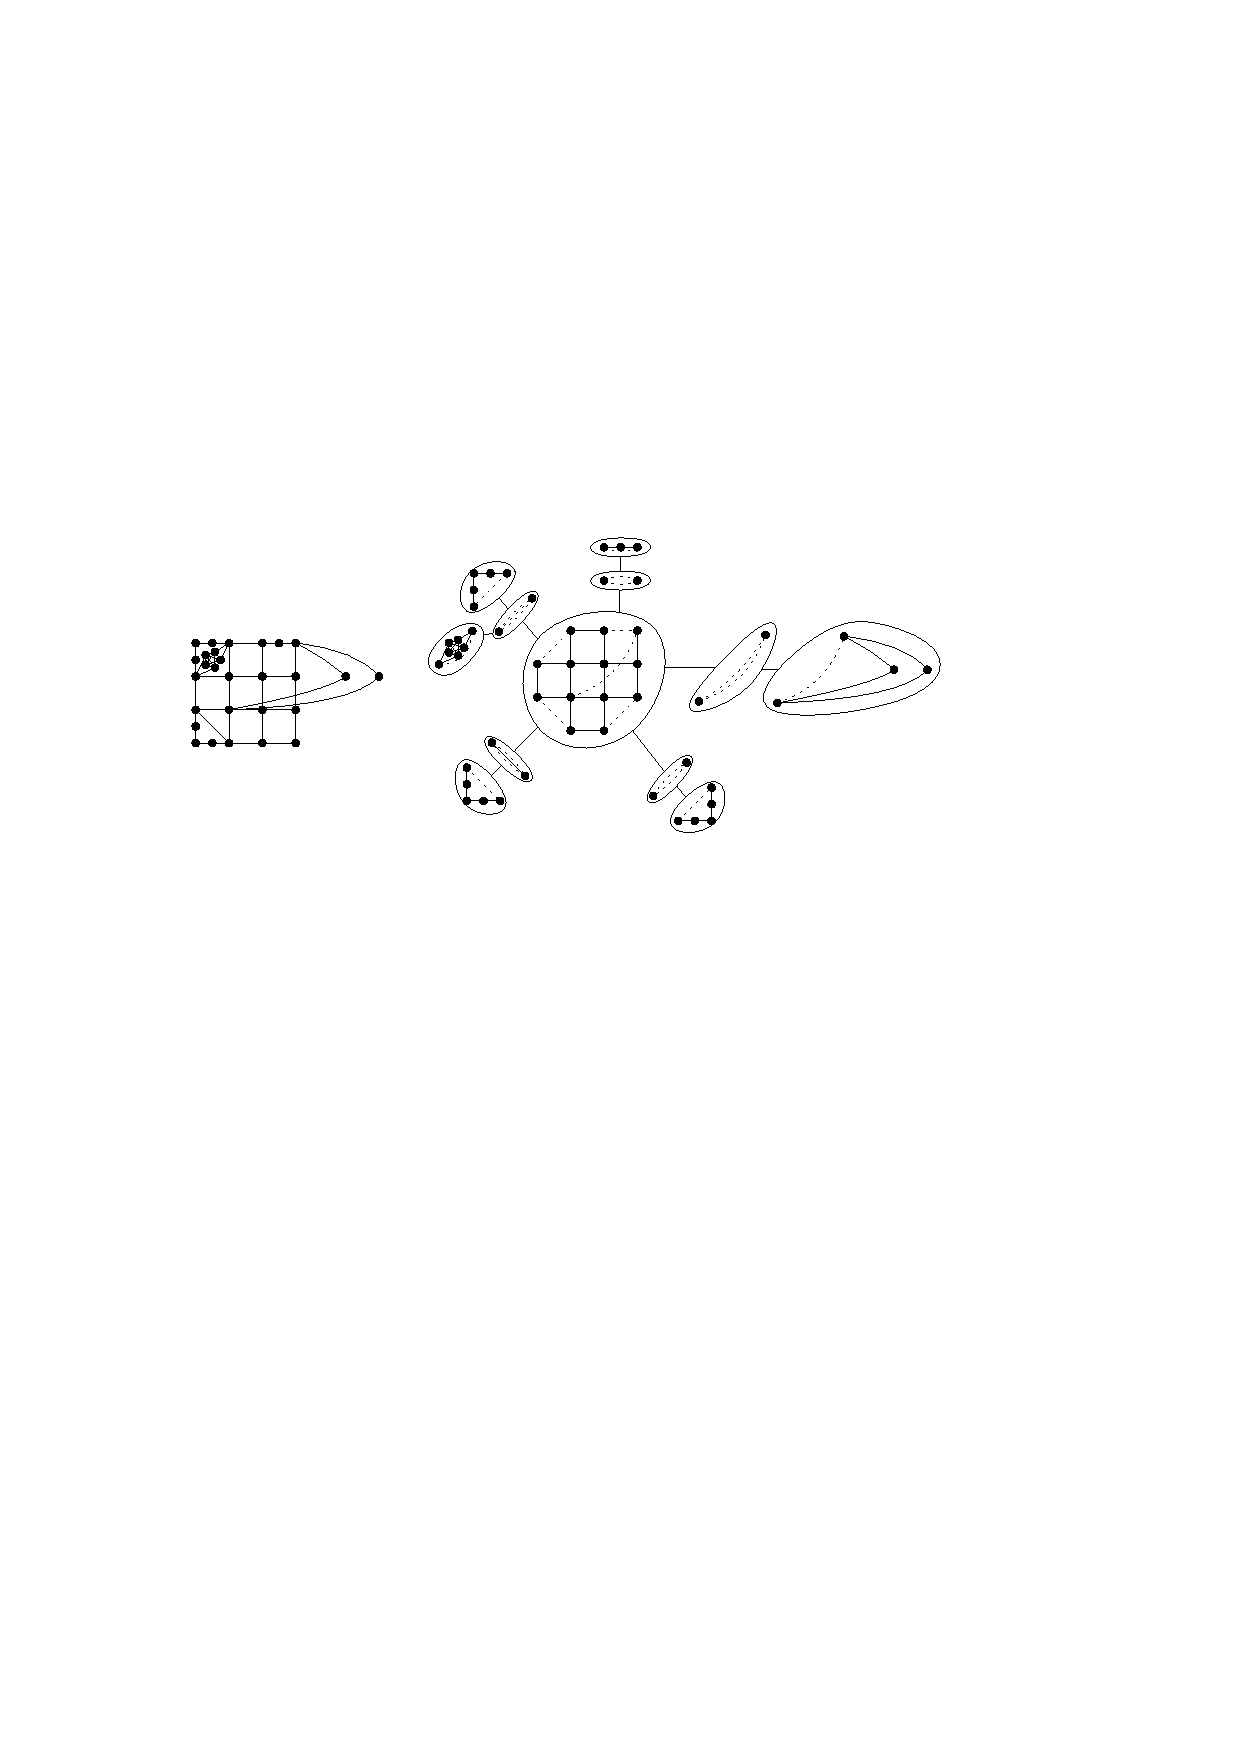
\includegraphics[width=\textwidth]{figs/spqr}
  \end{center}
  \caption{A graph and its SPQR-tree.}
  \label{spqr}
\end{figure}
\begin{enumerate}
   \item If $G$ is a cycle, then $S$ consists of a single node $a$
     (an S-node) in which $H_a=G$ and all edges of $H_a$ are real.

   \item If $G$ is 3-connected, then $S$ consists of a single node $a$
     (an R-node) in which $H_a=G$ and all edges of $H_a$ are real.  

%   \item If $G$ has an edge $xy$ such that $\{x,y\}$ is a cutset,
%     then let $C_1,\ldots,C_r$ be the connected components of $G-\{x,y\}$.
%     For each $i\in \{1,\ldots,r\}$, let $G_i=G[V(C_i)\cup\{x,y\}]$.
%     Note that each $G_i$ is 2-connected, so each has an SPQR-tree $S_i$.
%     Then the SPQR-tree for $G$ is obtained by creating a node $a$ (a
%     P-node) with $H_a$ being a \emph{dipole graph} having vertices $x$
%     and $y$ and having $k$ virtual edges joining $x$ and $y$ and one
%     real edge $xy$.  Now the edge $xy$ appears in each $S_i$ as a real
%     edge in exactly one node $a_i$ of $S_i$.
%     To complete $S(G)$ we make $a$ adjacent to each of $a_1,\ldots,a_k$ and we
%     make the edge the $xy$ a virtual edge in each of $H_{a_1},\ldots,H_{a_k}$.
%
%   \item Otherwise $G$ has a cutset $\{x,y\}$ such that $xy\not\in E(G)$
%     and $x$ and $y$ each have degree at least 3.
%     Then let $C_1,\ldots,C_r$ be the connected components of
%     $G-\{x,y\}$.  For each $i\in \{1,\ldots,r\}$, let $\tilde{G}_i$
%     be $G[V(C_i)\cup\{x,y\}]$ along with the additional edge $xy$.
%     Note that (because of the inclusion of $xy$) each $\tilde{G}_i$  is
%     2-connected, so each has an SPQR-tree $S_i$.  Then the SPQR-tree
%     for $G$ is obtained by creating a node $a$ (a P-node) with $H_a$
%     being a dipole graph with vertices $x$ and $y$ and having $k$
%     virtual edges joining $x$ and $y$.  Now the edge $xy$ appears in each
%     $S_i$ as a real edge in exactly one node $a_i$ of $S_i$.  To complete
%     $S(G)$ we make $a$ adjacent to each of $a_1,\ldots,a_k$ and we make
%     the edge the $xy$ a virtual edge in each of $H_{a_1},\ldots,H_{a_k}$.

   \item Otherwise $G$ has a cutset $\{x,y\}$ such that 
     $x$ and $y$ each have degree at least 3.
     Then let $C_1,\ldots,C_r$, $r\ge 2$, be the connected components of
     $G-\{x,y\}$.  For each $i\in \{1,\ldots,r\}$, let $\tilde{G}_i$
     be $G[V(C_i)\cup\{x,y\}]$ along with the additional edge $xy$.
     Note that (because of the inclusion of $xy$) each $\tilde{G}_i$  is
     2-connected, so each has an SPQR-tree $S_i$.  Then the SPQR-tree
     for $G$ is obtained by creating a node $a$ (a P-node) with $H_a$
     being a dipole graph with vertices $x$ and $y$ and having $k$
     virtual edges joining $x$ and $y$. In addition to these virtual edges, 
     $H_a$ contains
     the real edge $xy$ if $xy\in E(G)$.  The construction and the fact
     that $xy$ is an edge in each $\tilde{G}_i$ imply that there exists
     exactly one node $a_i$ in $S_i$ such that $xy$ is a real edge in
     $H_{a_i}$.
     To complete
     $S$ we make $a$ adjacent to each of $a_1,\ldots,a_k$ and we make
     the edge $xy$ a virtual edge in each of $H_{a_1},\ldots,H_{a_k}$.

\end{enumerate}

Let $S$ be the SPQR-tree of a 2-connected graph $G$.
For each node $a$ of $S$, we let $E_r(H_a)$ denote the set of real
edges in $H_a$ and $E_v(H_a)$ denote the multiset of virtual edges
in $H_a$.  For a connected subtree $S'$ of $S$ we define $G[S']$ as
the subgraph of $G$ whose vertex set is $V(G[S'])=\bigcup_{a\in V(S')}
V(H_a)$ and whose edge set is $E(G[S'])=\bigcup_{a\in V(S')} E_r(H_a)$.
For a vertex $v\in V(G)$, we denote the subtree of $S$ induced by $v$
as $S[v]=S[\{a\in V(S): v\in V(H_a)\}]$. 
We make use of the following properties of $S$:

\begin{enumerate}
   \item Every R-node and S-node is adjacent only to P-nodes and no two
   P-nodes are adjacent.
   \item The degree of any node $a$ is equal to the number of virtual edges
     in $H_a$.
   \item For every vertex $v\in V(G)$, $S[v]$ is connected.
   \item If $a$ is an R-node or S-node, then $H_a$ is a simple graph, i.e., $H_a$ does not contain any parallel edges.
   \item If a P-node $a$ has degree 2 and both its neighbors are S-nodes 
      then $H_a$ has a real edge.
%   \item For every 2-vertex cutset $\{x,y\}$ in $G$ there is at most
%     one P-node $a$ for which $V(H_a)=\{x,y\}$.
    \item For any node $a$ of $S$ and any component $S'$ of $S-\{a\}$,
     $G[S']$ is connected.
%   \item If $S'$ and $S''$ are two subtrees of $S$ that are adjacent to
%     but not including a common P-node $a$ whose dipole graph has vertices
%     $x$ and $y$, then $G[S']$ and $G[S'']$ have exactly two vertices,
%     $x$ and $y$ in common and have no edges in common.
   \item For each $xy\in E(G)$ there is exactly one node $a$ of $S$ 
    for which $xy$ is a real edge in $H_a$.
\end{enumerate}


\subsection{The Good Tree Decomposition}
\label{good-tree}

To obtain our good tree decomposition $(B_a:a\in V(T))$ of a 2-connected
graph $G$ we start with the SPQR-tree $S$ for $G$.  For each R-node
or S-node $a$ of $S$ we take a minimum-width path decomposition
$(B_c: c\in V(P_a))$ of $H_a$.  We say that the node $a$ \emph{generates}
the nodes in the path $P_a$ and that each node in $P_a$ is \emph{generated
by} $a$.

Each S- or R-node $a$ is adjacent to some set of P-nodes in $S$. For
each such P-node $b$ whose dipole graph $H_b$ has vertices $x$ and $y$, the edge $xy$ is a
(virtual) edge in $H_a$ and therefore $x$ and $y$ appear in some common
bag $B_c$ with $c\in V(P_a)$.  We make $c$ and $b$ adjacent in $T$. This defines
the tree $T$ in the tree decomposition. The contents of $T$'s bags are
obvious. Each P-node $a$ of $S$ becomes a node in $T$ whose bag contains
only the two vertices of $H_a$.  Every node $a$ in $T$ that is generated
by an S- or R-node $a'$ of $S$ is a node in some path decomposition of
$H_{a'}$ and already has an associated bag $B_{a}$
that it inherits from this path decomposition.

It is straightforward to verify that $(B_a:a\in V(T))$ is indeed a
tree decomposition of $G$: For any particular vertex $v\in V(G)$ the
connectivity of the subtree $T[v]$ follows from Property~3 of SPQR-trees and the equivalent property for the path decompositions that include $v$.
Each edge $xy$ of $G$ appears as an edge in $H_a$ for at least one node
$a$ of $S$ and therefore $x$ and $y$ appear in a common bag in the path
decomposition of $H_a$.

Each bag $B_a$ of $(B_a:a\in V(T))$ either has size in $\{2,3\}$
(when $a$ is generated by a P-node or an S-node) or it has size at
most $w(k)+1$ where $w(k)$ is the function in \cref{3-connected} (when
$a$ is generated by an R-node).  Thus, $(B_a:a\in V(T)\}$ is a tree
decomposition of $G$ whose width is upper bounded by a function of $k$.
What remains is to show that, for every $v\in V(G)$, $T[v]$ has pathwidth
that is upper bounded by a function of $k$.

In the remainder of this section, we fix $G$ to be a 2-connected graph,
$S$ to be the SPQR-tree of $G$ and $(B_a:a\in V(T))$ to be a tree
decomposition obtained using the procedure described above.  

\begin{lemma}
  \label{roof-lifting}
  For all integers $h\ge 1$,
  if $T[v]$ has pathwidth greater than $2^{2h+1}-3$, then $S[v]$ contains
  a subdivision of $T_h$.
\end{lemma}

\begin{proof}
  In a rooted binary tree we call the root and every degree 3 node
  \emph{branching nodes}.  Every branching node and every leaf is a
  \emph{distinctive node}.  We will use the convention that all binary
  trees are ordered, possibly arbitrarily, so that we can distinguish
  between the left and right child of a branching node.  For a node $a$
  in the rooted binary tree $T$, we denote by $\subtree{a}$ the subtree rooted
  at $a$, i.e., the subtree of $T$ containing all nodes that have $a$
  as an ancestor, including $a$ itself.

  Recall, from the result of \citet{BRST-JCTB91} discussed in the introduction,
  that if $T[v]$ has pathwidth greater than $2^{2h+1}-3$ then $T$
  contains a subdivision $T'$ of $T_{2h}$.  Note that $T'$ does not
  immediately imply the existence of $T_h$ in $S[v]$ since two or more
  distinctive nodes of $T'$ may have been generated by the same node of $S$.  
  Label each node of $T'$ with the node of $S$
  that generated it.  Recall that each node $a$ in $S$ generates a path
  in $T$ so, if we consider a maximal subset of nodes of $T'$ with a common
  label then this subset induces a path in $T'$.

  We claim that $T'$ contains a subdivision $T''$ of $T_{h}$ such that
  each of the distinctive nodes of $T''$ has a unique label.  We establish
  this claim by induction on $h$: If $h=0$ then the claim is trivial.
  Otherwise, let $a$ be the root of $T'$ and let $a'$ and
  $a''$ be the highest branching nodes in the left and right subtrees
  of $\subtree{a}$, respectively.  Let $a_1$ and $a_2$ be the highest
  distinctive nodes in the left and right subtrees of $\subtree{a}'$,
  respectively, and let $a_3$ and $a_4$ be the highest distinctive nodes in
  the left and right subtrees of $\subtree{a}''$, respectively.  Since each
  label induces a path in $T'$, at least
  one of $\{a_1,a_2\}$, say $a_1$, and at least one of $\{a_3,a_4\}$, say $a_4$, does not have the same label as $a$.
  Furthermore, since $a_1$ and $a_4$ are separated by $a$, the set of labels
  of nodes in $\subtree{a}_1$ is disjoint from the set of labels of
  nodes in $\subtree{a}_4$.  Applying induction on $\subtree{a}_1$
  and $\subtree{a}_4$ yields two subdivisions of $T_{h-1}$ in which
  each distinctive node has a unique label.  Connecting these two
  subdivisions with the unique path from $a_1$ to $a_4$ yields the
  desired subdivision of $T_{h}$ in which each distinctive node has
  a unique label.

  Now, each distinctive node in $T''$ has a unique label and therefore
  corresponds to a unique node of $S$.  Thus, if we contract all nodes of
  $T''$ sharing a common label, then we obtain a subtree $T'''$ of $S[v]$
  that is a subdivision of $T_{h}$.
\end{proof}

Thus far we have established that if $T[v]$ has sufficiently high
pathwidth, then $S[v]$ contains a subdivision of a large complete binary
tree.

\begin{lemma}\label{qk-minor}
  If $S[v]$ contains a subdivision of $T_{7(k+1)}$ then $G$ contains a 
  $Q_{k}$ minor.
\end{lemma}

\begin{proof}
  First we note that if $S[v]$ contains a subdivision of $T_{7(k+1)}$
  then $S[v]$ contains a subdivision $T'$ of $T_{k+1}$ such that the path
  between any pair of distinctive nodes in $T'$ has length at least 7.

  It is convenient to work with a simplified SPQR-tree $S'$ and graph $G'$
  obtained by repeating the following operation exhaustively: Consider
  some edge $ab$ of $S$ with $a\in V(T')$ and $b\not\in V(T')$. The edge
  $ab$ is associated with some virtual edge $xy$ in $H_a$.  In $S'$ we
  replace the virtual edge $xy$ in $H_a$ with a real edge. At the same
  time we remove the maximal subtree $\subtree{b}$ of $S$ that contains
  $b$ and not $a$. By Property~6 of SPQR trees, in $G'$ this operation
  is equivalent to contracting all the real edges in $\bigcup_{c\in
  V(\subtree{b})} E_r(H_c)$ and removing any resulting parallel edges.
  Since the resulting graph $G'$ is a minor of $G$, this operation is
  safe in the sense that the existence of a $Q_k$ minor in $G'$ implies
  the existence of a $Q_k$ minor in $G$.

  With this simplification, the tree $T'$ is the SPQR-tree for the
  graph $G'$ and every virtual edge is incident to $v$.  We now turn
  our efforts to finding the $Q_k$ minor in $G'$.  Recall that $Q_k$
  is the union of a complete binary tree $T_k$ and an apex vertex.
  We begin by finding a subdivision $T''$ of $T_{k+1}$ in $G'$. In this
  subdivision, each edge of $T_{k+1}$ that joins a node to its left child
  is represented by a path $P_{\mu\nu}$ joining a branching node $\mu$
  to a distinctive node $\nu$. We show that $G'$ contains a path from $v$ to some \emph{anchor node} $\eta$
  of $P_{\mu\nu}$ with $\eta\neq\nu$, which is vertex disjoint from $T''$ except for $\eta$.  Furthermore, except for their
  common endpoint $v$, all of these paths are disjoint. The union of $T''$
  and these paths contains a $Q_k$ minor since contracting the path from
  each anchor node to its closest ancestor branching node produces $Q_k$.
  See \cref{qk}.

  \begin{figure}
    \begin{center}
      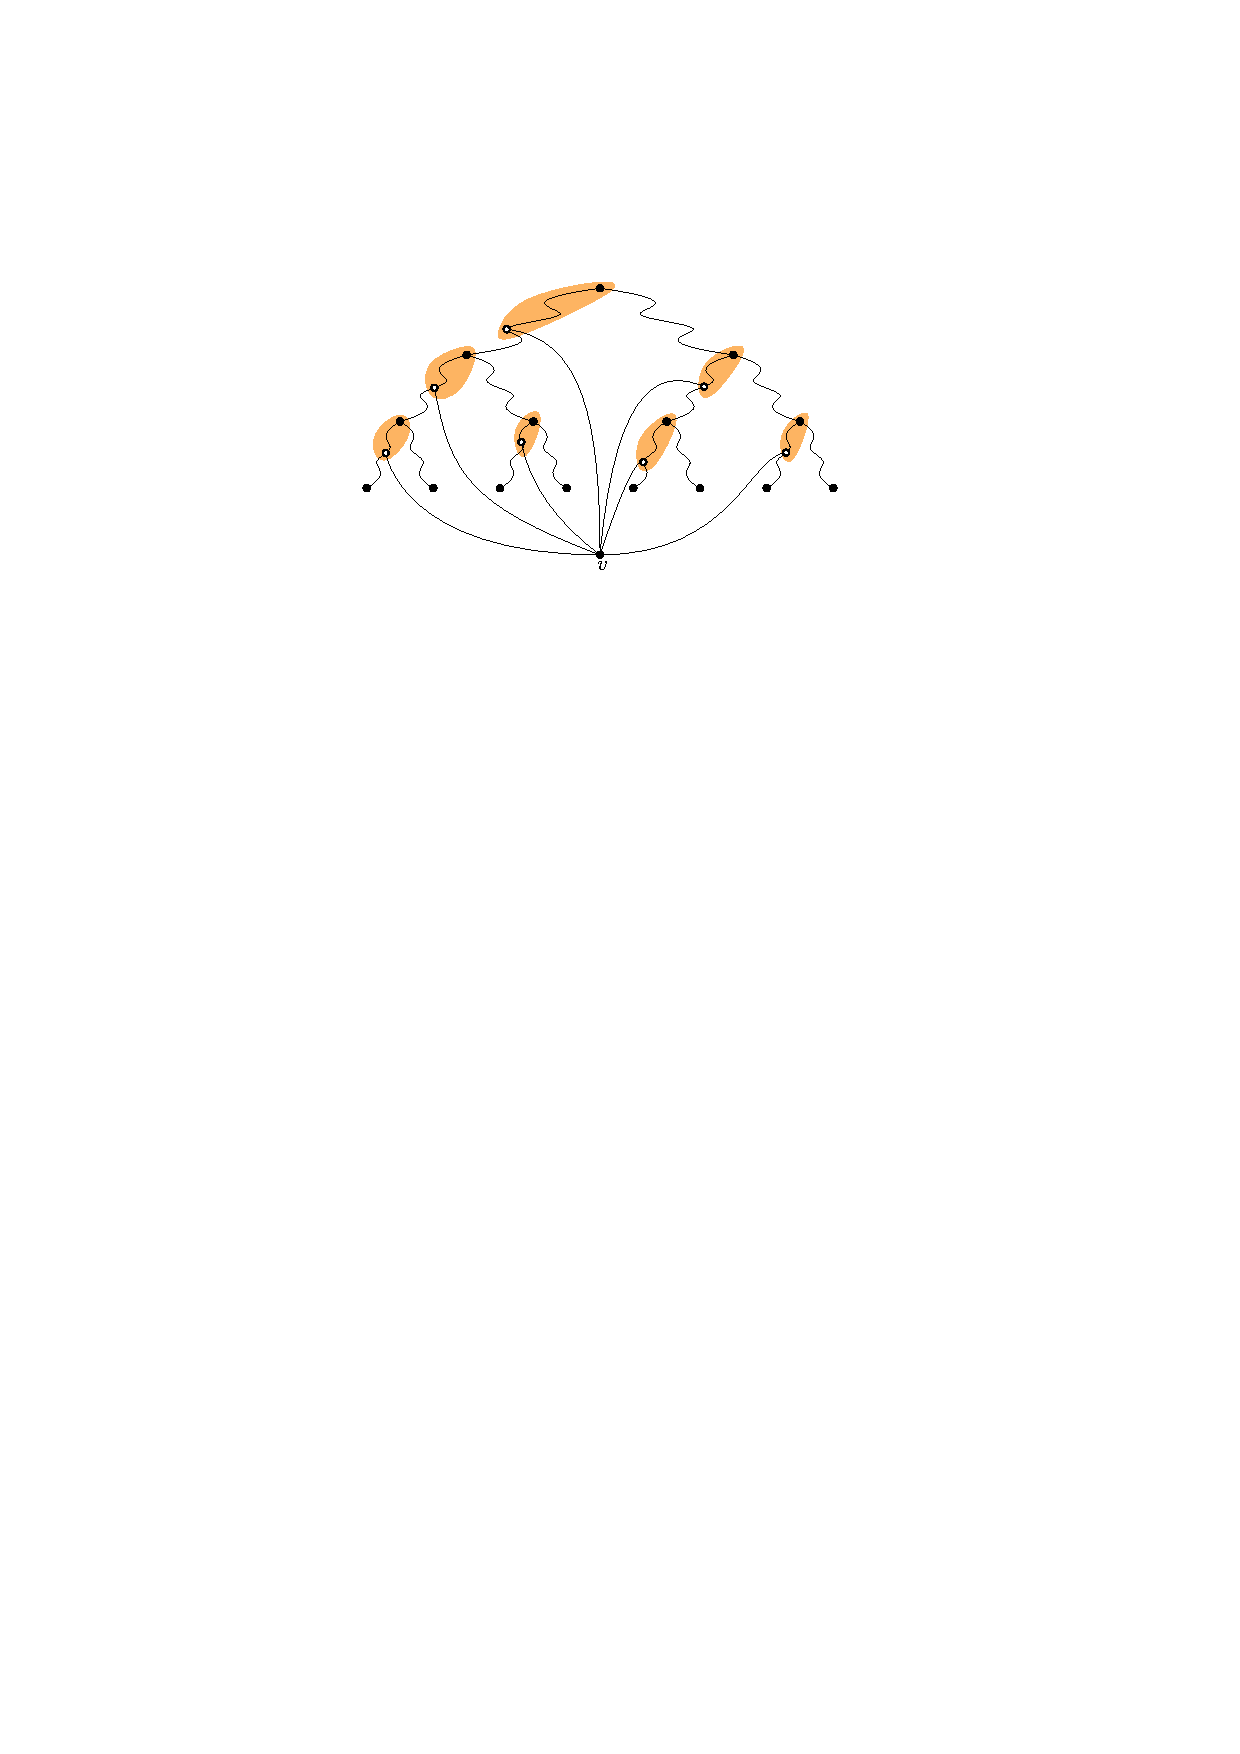
\includegraphics{figs/qk}
    \end{center}
    \caption{Finding a $Q_k$ minor in the proof of \cref{qk-minor}. Distinctive nodes are indicated by black disks and anchor nodes by white circles.}
    \label{qk}
  \end{figure}

  Let $a$ be a branching node of $T'$ and let $b$ be the nearest
  distinctive node in one of $a$'s two subtrees.  Consider the path
  $a=c_1,c_2,\ldots,c_r=b$ in $T'$.  For each $i\in\{1,\ldots,r-1\}$,
  the edge $c_ic_{i+1}$ is associated with a cutset $\{v,x_i\}$ in
  $G'$ and $vx_i$ is a virtual edge in $H_{c_i}$ and $H_{c_{i+1}}$.
  Note that this implies that, for each $i\in\{2,\ldots,r\}$, $H_{c_i}$
  contains both vertices $x_i$ and $x_{i-1}$.

  Refer to \cref{paths}.  We claim that, for each $i\in\{2,\ldots,r-1\}$,
  $H_{c_{i}}$ contains a path $P_i$ from $x_{i-1}$ to $x_{i}$ that
  does not contain $v$.  When $c_i$ is a P-node, this claim is trivial
  since, in this case, $x_{i-1}=x_{i}$.  The case in which $c_i$
  is an S-node or R-node is also easy: In these cases $H_{c_i}$ is
  2-connected, therefore there is a path from $x_{i-1}$ to $x_{i}$
  that avoids $v$.  Now note that the paths $P_1,\ldots,P_{r-1}$ are
  disjoint, except for each of the common endpoints $x_i$ where $P_{i}$ ends and $P_{i+1}$ begins.  This is because each $\{v,x_i\}$ is 
  a cutset of $G'$ that
  separates $\bigcup_{j=1}^{i} V(H_{c_j})\setminus\{v,x_i\}$ from
  $\bigcup_{j={i+1}}^r V(H_{c_j})\setminus\{v,x_i\}$.  By concatenating
  $P_2,\ldots,P_{r-1}$ we obtain a path $P_{ab}$ from $x_1\in V(H_a)$
  to $x_{r-1}\in V(H_b)$ that we call the \emph{subdivision path} for
  nodes $a$ and $b$.

  \begin{figure}
    \begin{center}
      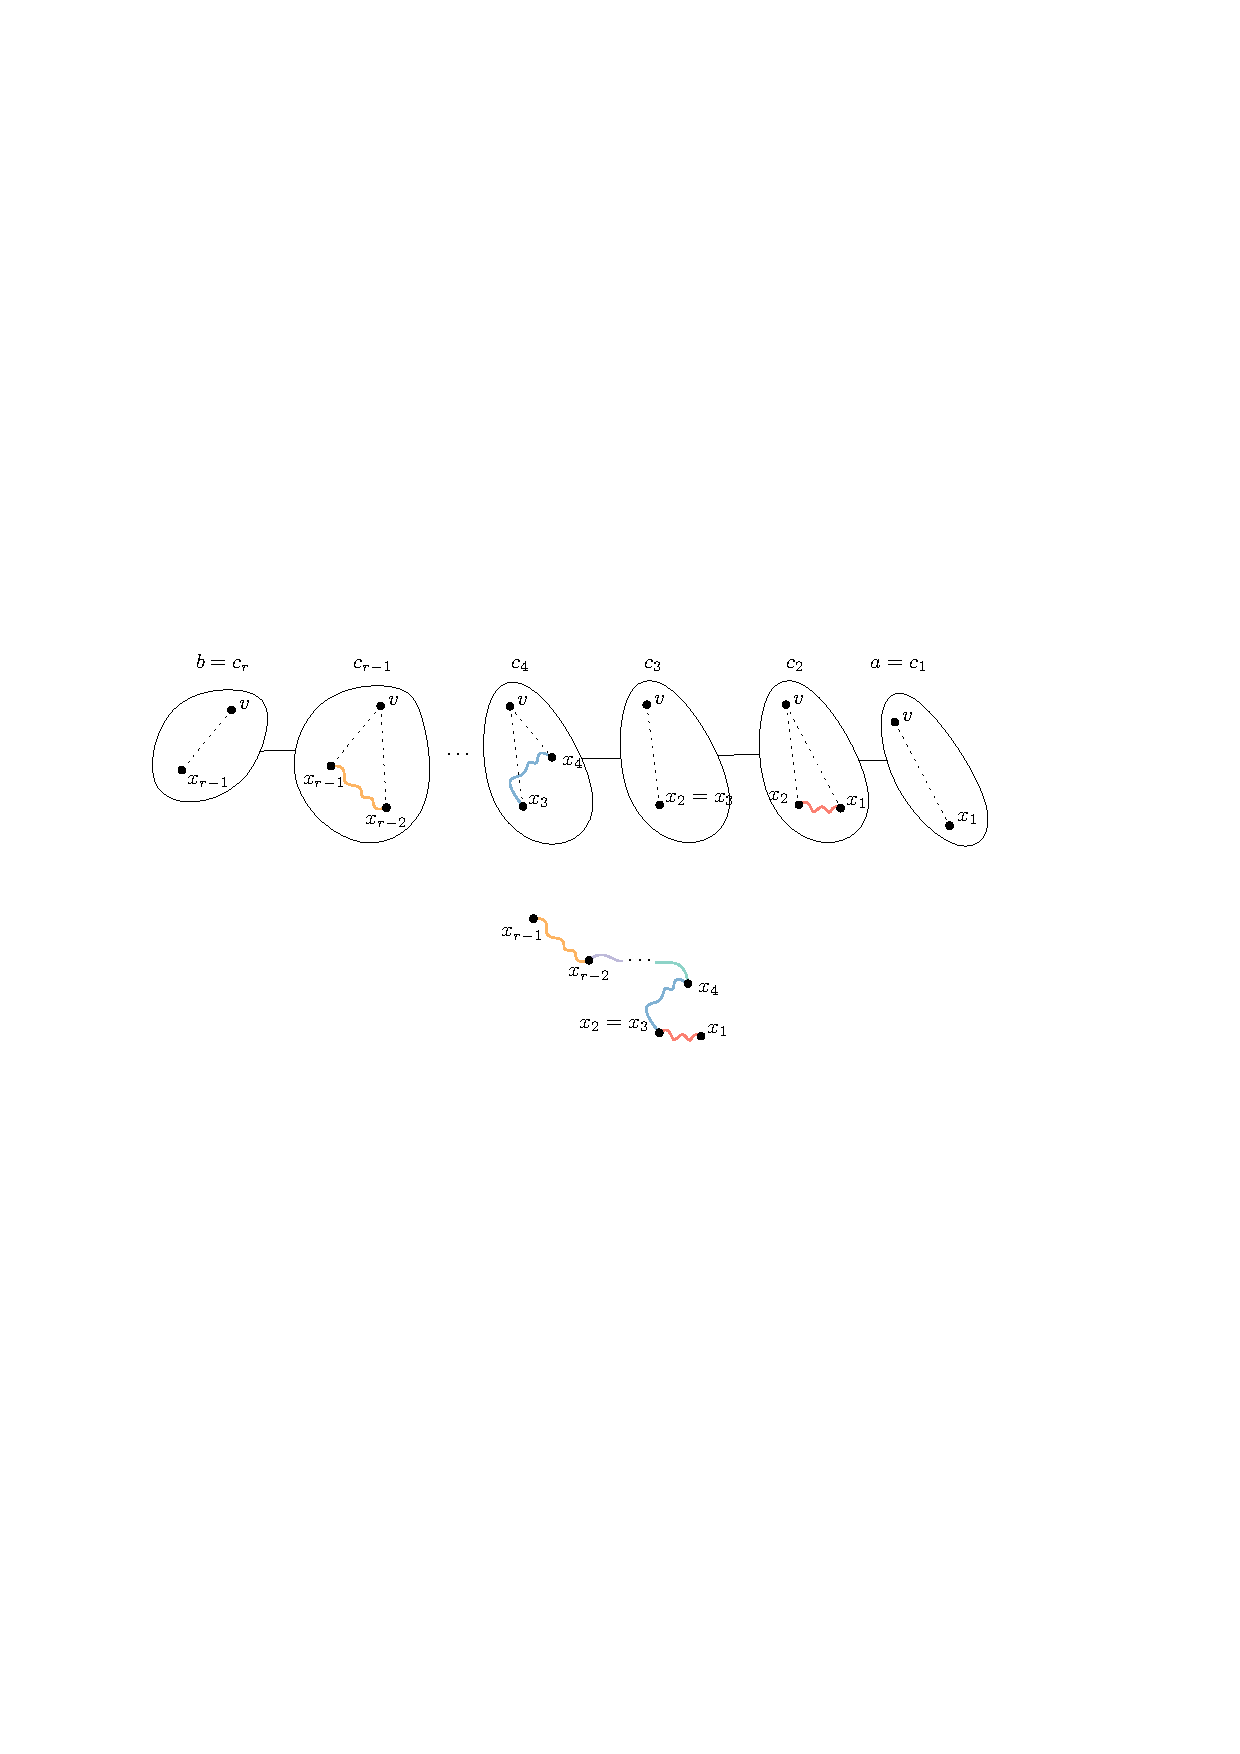
\includegraphics{figs/paths}
    \end{center}
    \caption{Finding a path connecting a vertex of $H_a$ to a vertex of $H_b$.}
    \label{paths}
  \end{figure}

  By Properties~2 and 4 of SPQR-trees and the fact that all virtual
  edges are incident to $v$, every branching node $a$ of $T'$ is either
  an R-node or a P-node. In the case where $a$ is a P-node, all the
  subdivision paths that begin or end at a vertex of $H_a$ include
  the same vertex of $H_a$.  In the case where $a$ is an R-node, each
  subdivision path that begins or ends at a vertex of $H_a$ includes
  a different vertex (for up to 3 different vertices $x$, $y$, and
  $z$). Now, since $H_a$ is 3-connected, these three vertices are in the
  same component of $H_{a}-\{v\}$. In particular, $H_a-\{v\}$ contains
  an edge-minimal tree that includes $x$, $y$, and $z$.  Adding each
  of these trees to the union of all subdivision paths produces the
  subdivision $T''$ of $T_{k+1}$.

  Next we show how to construct paths from $v$ to anchor nodes.
  Let $a$ be a branching node of $T'$, let $b$ be the highest
  distinctive node in $a$'s left subtree and let $c_1=a,\ldots,c_r=b$
  be the path in $T'$ having endpoints $a$ and $b$.   
  Thus far we have established
  that $G'[\{c_2,\ldots,c_{r-1}\}]$ contains a simple path $P_{ab}$
  from $x_1$ to $x_{r-1}$ that does not include $v$.    We now show
  that $G'[\{c_2,c_3,c_4,c_5\}]$ contains an \emph{apex path} $P'$
  from $v$ to some \emph{anchor node} of $P_{ab}$ such that the
  internal vertices of $P'$ are disjoint from $V(P_{ab})\cup V(H_{b})$.
  We first describe the path $P'$ in $G'[\{c_2,c_3,c_4,c_5\}]$ and then
  show that $P'$ does not contain any vertex of $V(H_b)\setminus\{v\}$.
  There are two cases to consider:
  \begin{enumerate}
    \item $c_i$ is an R-node, for some $i\in\{2,\ldots,5\}$:  Since
    $H_{c_i}$ is 3-connected, there are three paths in $H_{c_i}$
    with endpoints $v$ and $x_i$ and no other vertices in common.
    Since $H_{c_{i}}$ has only two virtual edges, at least one of these
    paths uses only real edges in $H_{c_i}$.  This path therefore
    contains a subpath $P'$ joining $v$ to some vertex of $P_{ab}$
    (the anchor vertex) that is otherwise disjoint from $P_{ab}$.

    \item Otherwise, none of $c_2,\ldots,c_5$ is an R-node. Property~1
    of SPQR-trees implies that, for at least one $i\in\{2,3\}$, $c_i$ is
    an S-node, $c_{i+1}$ is a P-node and $c_{i+2}$ is an S-node.  But in
    this case, Property~5 of SPQR-trees ensures that $H_{c_{i+1}}$
    contains the real edge $vx_{i+1}$. Therefore, in this case there is a
    single edge path $P'$ from $v$ to $P_{ab}$.
  \end{enumerate}
  It remains to show that $P'$ does not contain any vertices of
  $V(H_b)\setminus \{v\}$.  By Properties~1 and 6 of SPQR-trees,
  for any $x\in V(G')\setminus\{v\}$, the subtree $T'[x]$ of $T'$
  consisting only of nodes $a$ such that $x\in V(H_a)$ is a star, i.e.,
  the distance between any two nodes in $T'[x]$ is at most 2.  Now,
  since the distance between any two distinctive nodes of $T'$ is at least
  $7$, $r\ge 8$ and therefore $H_b=H_{c_r}$ has no vertex, except $v$,
  in common with any of $H_{c_2},\ldots,H_{c_5}$.  Therefore, $P'$
  joins $v$ to a vertex in $P_{ab}$ that is not in $H_{b}$, as required.

  Adding the set of all apex paths to $T''$ then produces a subgraph of
  $G'$ that contains a $Q_k$-minor.
\end{proof}

%\comment{ With a little more careful analysis in the preceding proof, the $7(k+1)$ that appears everywhere could be reduced to $6(k+1)$. Does anyone care? GJ: No. DW: no}

%\comment{The requirement that $S[v]$ contains a subdivision of $T_{7(k+1)}$ is quite a bit stronger than necessary.  It is enough if $S[v]$ contains a subdivision of a 6-subdivision of $T_{k+1}$.  This would reduce the pathwidth dependence in the next proof from $2^{14(k+1)}-3$ down to $7\cdot 2^{2(k+1)}-3$. (Even the leading 7 could be reduced further.) GJ: What about stating we do not try to optimize constants (and keep current proof)? DW: I agree with GJ.}

\comment{Let $Q^*_k$ be the graph (shown in \cref{qk}) obtained by subdividing each edge of $T_{k+1}$ and adding a vertex $v$ adjacent to all subdivision vertices. The proof above actually shows that, if $S[v]$ contains a subdivision of $T_{9(k+1)}$ then $G$ contains a \emph{subdivision} of $Q^*_k$.  This is a little bit surprising, since I would have guessed that $v$ would have to be a contracted subgraph of $G$, not a single high-degree vertex. Is it worth writing the proof to highlight this? GJ: Yes it is surprising at first sight. Note that in the $R$-nodes we do need to forbid $Q_k$ as a minor, not enough to forbid a $Q^*_k$-subdivision. So there the minor relation is needed. }

Finally, we have all the pieces in place to complete the proof.

\begin{proof}[Proof that (1) implies (5)]
Let $G$ be a graph excluding some apex-forest graph $H$ as a minor. As explained earlier, $G$ contains no $Q_k$ minor for some $k=k(H)$.  We wish to show that there are $w$ and $p$ that depend only on $k$ such that $G$ has a $(w,p)$-good tree decomposition.  By \cref{cut-vertices} we may assume that $G$ is 2-connected.

Consider the good tree decomposition $(B_a:a\in V(T))$ of $G$ described in   \cref{good-tree}.    This decomposition has width at most $w$ where   $w=w(k)$ is the function that appears (implicitly) in \cref{dang-theorem} and \cref{3-connected}.   We claim that, for each $v\in V(G)$, $\pw(T[v])\le   2^{14(k+1)}-3$, so that this tree decomposition is   $(w,2^{14(k+1)}-3)$-good.  Otherwise, by \cref{roof-lifting}, there is a vertex $v\in V(G)$ such that the SPQR-tree $S$ has a subtree $S[v]$ that contains a subdivision of $T_{7(k+1)}$.  Therefore, by \cref{qk-minor}, $G$ contains a $Q_k$ minor, contradicting the supposition that $G$ has no $Q_k$ minor.
\end{proof}


\comment{Depending on where we decide to submit this paper, we may want
to discuss algorithmic complexity, which the following theorem sketches.\\DW: I vote to keep this.}

\begin{theorem}
   There exists a function $f:\mathbb{N}\to\mathbb{N}$ and an algorithm
   that takes as input an $n$-vertex graph and outputs, in $O(f(k)n)$
   time, an $(f(k),f(k))$-good tree decomposition of $G$ and a layered
   path decomposition of $G$ of layered width at most $f(k)$, where $k$
   is largest integer such that $G$ contains a $Q_k$ minor.
\end{theorem}

\begin{proof}
   In the following, for each $i\in\{0,\ldots,5\}$,
   $f_i:\mathbb{N}\to\mathbb{N}$ is an unspecified function that is known
   to exist.  The fact that $G$ has no $Q_k$-minor implies that the number
   of edges of $G$ is at most $f_0(k)n$ (see \citep{ReedWood16}).  
   Computing the SPQR-tree $S$ of $G$ can
   be done in $O(f_0(k)n)$ time and the total size of the graphs $\{H_a:a\in
   V(S)\}$ is at most $f_0(k)n$ (see \cite{GM00}).  Computing a path decomposition of
   $H_a$ with width at most 2 for each S-node or P-node $a$ is easily
   done in time linear in the size of $H_a$.  For each R-node $a$, the
   pathwidth of $H_a$ is at most $p=p(k)=O(1)$.  Therefore, computing
   a minimum-width path decomposition of $H_a$ for an R-node $a$ can be
   done in $O(f_1(k)|V(H_a)|)$ time \cite{Bod93,BK91,K93,CDF96,Bodlaender-SJC96}. These
   path decompositions are all that is needed to construct the tree $T$
   and an $(f_2(k),f_3(k))$-good tree decomposition $\{ B_a:a\in V(T)\}$
   in $O(f_1(k)n)$ time.

\comment{DW: I would delete reference \citep{Bod93}, since \citep{Bodlaender-SJC96} is the updated journal version.}

   The proof that (5) implies (4) in \cref{easy-section} is constructive
   and immediately gives an $O(f_4(k)n)$ time algorithm to convert
   the $(f_2(k),f_3(k))$-good tree decomposition into a layered path
   decomposition of layered width at most $f_5(k)$. This establishes the
   theorem for $f(k) = \max\{f_i(k) : i\in\{1,\ldots,5\}\}$.
\end{proof}

%\textcolor{red}{It remains to prove that (1) implies (4), or (2) implies (4). }
%
%\section{New Stuff} 
%
%Short version: We think we have all the necessary ingredients to
%finish the paper now, thanks to a recent result of Thanh Dang, a
%student of Robin Thomas, who characterized unavoidable minors in
%3-connected graphs of large pathwidth in his PhD thesis. A corollary
%of his main result is that 3-connected graphs with no $Q_k$ minor have
%bounded pathwidth, where $Q_k$ is the complete binary tree of height $k$ plus a 
%universal vertex.
%
%Long version, with recaps of previous stuff:
%
%- Say G is a graph with no $Q_k$-minor (or equivalently, $G$ and all its
%minors have bounded local pathwidth)
%
%- The missing part in our draft was a proof that $G$ has bounded layered pathwidth
%
%- We know it is enough to show that $G$ has a 'good tree decomposition',
%a tree decomposition of bounded width such that, for each vertex $v$ of
%$G$, the corresponding subtree $T_v$ has bounded pathwidth
%
%- To show this, we may easily reduce to the 2-connected case, so
%assume $G$ is 2-connected
%
%- To handle the 2-connected case, David Eppstein\ suggested to look at the
%associated SPQR-tree and study how the triconnected components of a
%graph can be 2-summed together without ever creating a $Q_k$ minor
%
%- In a series of emails (April 2015), he showed the following:
%
%** Say that an R-node is 'safe' if, in the corresponding 3-connected
%graph, either there are at most 2 virtual edges, or there are three
%virtual edges and they form a triangle, or the graph is obtained from
%a planar graph with all virtual edges are on a common face using
%3-sums with other 3-connected graphs
%
%** In a safe R-node, it is not possible contract edges of the
%corresponding graph so as to have three parallel virtual edges
%
%** Conversely, in an unsafe R-node, it is always possible to do so.
%(The intuition is that unsafe R-nodes allow some kind of branching of
%2-cutsets while safe R-nodes don't.)
%
%** If the SPQR-tree of G contains a subdivision of a large enough
%complete binary tree such that the degree-3 nodes are either P-nodes
%or unsafe R-nodes, then there is a $Q_k$-minor in $G$
%
%** So this does not happen, and using this we can reduce to the
%3-connected case: Assuming that we have a good tree decomposition of
%each triconnected component of G, we can join them together following
%the 2-sums encoded by the SPQT-tree and argue that the pathwidth of
%our subtrees $T_v$ does not explode, otherwise we would find the
%complete binary tree from the previous step.
%
%- To show that the triconnected components have good tree
%decompositions, it is enough to show that a 3-connected graph with no
%$Q_k$ minor must have bounded pathwidth
%
%- This is a corollary of Theorem 1.1.5 on page 3 in thesis of  \citet{Dang18}:
%
%** In that theorem, choose $P'$ to be the complete binary of height k
%plus two universal vertices. Choose $Q'$ to be the "universal"
%outerplanar graph of depth $k+1$, as defined in \cite[page 3]{HJMW}, plus one universal
%vertex. Choose $R'$ to be the complete binary of height $2^k +1$ plus a
%cycle on its leaves.
%
%** Clearly, $P'$ contains $Q_k$ as a minor
%
%** Q' also does, because $U_{k+1}$ contains a complete binary of height
%k as a subgraph
%
%** Finally, R' also contains a $Q_k$ minor: Contract the cycle, then we
%have a complete binary tree of height $2^k$ plus an apex vertex linked
%to its leaves, which contains $Q_k$ as minor (see e.g. \citep[Lemma 2.2 on page 4]{HJMW}.
%
%
%\section{SPQR Trees --- from Wikipedia}
%
%An SPQR tree is an unrooted tree in which for each node $x$ there is associated an undirected graph or multigraph $G_x$. The node, and the graph associated with it, may have one of four types, given the initials SPQR:
%
%In an S node, the associated graph is a cycle graph with three or more vertices and edges. 
%
%In a P node, the associated graph is a dipole graph, a multigraph with two vertices and three or more edges. 
%
%In a Q node, the associated graph has a single real edge. This trivial case is necessary to handle the graph that has only one edge. In some works on SPQR trees, this type of node does not appear in the SPQR trees of graphs with more than one edge; in other works, all non-virtual edges are required to be represented by Q nodes with one real and one virtual edge, and the edges in the other node types must all be virtual.
%
%In an R node, the associated graph is a 3-connected graph that is not a cycle or dipole. 
%
%Each edge $xy$ between two nodes of the SPQR tree is associated with two directed virtual edges, one of which is an edge in $G_x$ and the other of which is an edge in $G_y$. Each edge in a graph $G_x$ may be a virtual edge for at most one SPQR tree edge.
%
%An SPQR tree T represents a 2-connected graph $G-T$, formed as follows. Whenever SPQR tree edge $xy$ associates the virtual edge $ab$ of $G_x$ with the virtual edge $cd$ of $G_y$, form a single larger graph by merging $a$ and $c$ into a single supervertex, merging $b$ and $d$ into another single supervertex, and deleting the two virtual edges. That is, the larger graph is the 2-clique-sum of $G_x$ and $G_y$. Performing this gluing step on each edge of the SPQR tree produces the graph $G_T$; the order of performing the gluing steps does not affect the result. Each vertex in one of the graphs $G_x$ may be associated in this way with a unique vertex in $G_T$, the supervertex into which it was merged.
%
%Typically, it is not allowed for two S nodes to be adjacent, nor for two P nodes to be adjacent, because if such an adjacency occurred the two nodes could be merged into a single larger node. With this assumption, the SPQR tree is uniquely determined from its graph. When a graph G is represented by an SPQR tree with no adjacent P nodes and no adjacent S nodes, then the graphs $G_x$ associated with the nodes of the SPQR tree are known as the triconnected components of $G$.
%
%\section{Comment by David Eppstein, 8 April 2015}
%
%Something still seems strange to me about your proposed structure theorem for minor-closed families of bounded local pathwidth. For the other restricted structure theorems (for families excluding a planar graph, families excluding a one-crossing graph, families excluding a tree, etc) we have a characterization that itself gives a minor-closed family (graphs of bounded treewidth, clique-sums of planar graphs and graphs of bounded treewidth, graphs of bounded pathwidth, etc). But your proposed structure, a tree decomposition of low width in which each vertex belongs to a set of bags of low pathwidth, is not minor-closed. For instance, let T be a large binary tree and consider the graph G = K2 x T. Then G has a tree decomposition that is itself in the form of a large binary tree, with each vertex belonging to a three-bag path formed by a parent and its two children, so it fits your structure theorem. But if you collapse one of the two copies of T in G, you get a large tree-apex graph. This suggests to me that, although your conjecture that this structure might always exist should still be true, there is a more highly constrained structure that always exists and might be easier to prove.
%
%For a while I thought maybe the structure might be the following: let F be a minor-closed family of bounded local pathwidth; then I thought the graphs in F would necessarily be 1-sums of graphs of bounded pathwidth. But this is too constrained and turns out to be false. The outerplanar graphs do not have this form, but every outerplanar graph has bounded local pathwidth (did you already know this?). Here's a construction of a layered pathwidth 2 layering of an arbitrary outerplanar graph: find a one-page book embedding of the graph (in a halfspace), and label every vertex and face by its distance in the vertex-face incidence graph from the (unique) unbounded face of the embedding. Use the vertex labels as layers; every two adjacent vertices share a face, so they can have labels at most two units apart and therefore are either on the same layer or on consecutive layers. Make a path decomposition as follows: for each vertex (in left to right order), make a bag containing that vertex and the vertex closest to it on the left with each label (including its own label). I've attached a figure showing the construction.
%
%So now I'm wondering what the right kind of structure is. It should allow arbitrary 1-sums, outerplanar graphs, and bounded-pathwidth graphs, but it's also possible to do some (but not arbitrary) 2-sums or 3-sums between the bounded-pathwidth pieces and the outerplanar pieces in a controlled way that preserves the hereditary bounded local pathwidth. And unlike your proposed structure, every minor of every graph with this structure should have bounded local pathwidth.
%
%
%\section{Comment by David Eppstein 9 April 2015}
%
%So in connection with this I've been looking today at the structure of 2-connected graphs (their SPQR trees) when their minors have bounded local pathwidth. I think, for instance, that if you take a collection of planar graphs of bounded pathwidth, and then you 2-sum them together in such a way that
%- each edge is used to 2-sum only two of the graphs
%- within each of the planar graphs, the edges used for 2-sums all lie on a single face
%then the result should still have minor-closed bounded local pathwidth, regardless of the shape of the SPQR tree.
%
%On the other hand if there is a subdivision of a large complete binary tree within the SPQR tree such that each of the branching nodes of the subdivision is either
%- a P node, or
%- an R node that can be contracted to a P node (i.e. you can contract its graph down to a two-vertex bipole multigraph keeping each of the three 3-sum edges uncontracted)
%then you can use this to form a minor in the form of a Cartesian product of large tree T with K2, and then contracting one of the two copies of T gives a large apex-tree minor.
%
%These two constructions show that we can't just look at the SPQR tree, and at the pathwidth of the 3-connected components, to determine whether a graph has minors with bounded local pathwidth. We have to look inside the 3-connected components to see how they're connected to the rest of the SPQR tree.
%Because we could have two graphs with isomorphic SPQR trees that are large binary trees of R nodes, but where the R nodes of one graph are bounded-pathwidth planar graphs with its 2-sums all on the same face, and the R nodes of the other can be contracted to P nodes. Despite having the same SPQR tree, the first graph would have minors with bounded local pathwidth and the second wouldn't.
%
%Based on this I'd like to understand when a 3-connected graph plus three designated edges can be contracted down to a bipole multigraph and when it can't. The situation of a planar graph with all three edges on one face is an example when it can't, because any contraction preserves the fact that the three edges still lie on a single face. Another example is an arbitrary 3-connected graph in which the three edges form a triangle. And if G is a graph with three designated edges that cannot be contracted down in this way, then any clique-sum of G with another graph doesn't change anything. Are those the only possibilities?
%
%\section{Comment by David Eppstein 14 April 2015}
%
%Recall from my earlier message that if the SPQR tree contains a subdivision of a ternary tree T in which the branching nodes are either P nodes or R nodes that can be contracted to P nodes, then the graph can be contracted to K2 x T (actually not quite, for each edge of T one of the two copies of the edge in K2 x T could be contracted) and then by collapsing one of the copies of T we can find a large tree-apex minor. This gives a way for a graph to fail to have minor-closed bounded local pathwidth even when each of its 3-connected components is individually well-behaved, and maybe the only way for it to fail. So I'm still trying to investigate the conditions under which an R node (3-connected component) can be contracted to a P node (multigraph with two vertices and three edges, in which the three uncontracted edges are the virtual edges linking the R node to other parts of the SPQR tree).
%
%The case when the three virtual edges in the R node form a triangle is easy (it can't be contracted to a P node) and the case in which they form a claw is almost as easy (it can always be contracted). The next simplest case is when they form a three-edge path. In this case, I believe the result is that the R node can be contracted into a P node if and only if the 3-connected component is not a planar graph with the path forming part of a face, and is not a graph obtained from a planar graph (with the path on a face) by 3-sums with other graphs.
%
%The key lemma (which I imagine is likely known somewhere in Robertson and Seymour's many papers on this sort of thing): suppose G is a 4-connected graph with four designated vertices p,q,r,s. Then either (1) G is planar and pqrs are on one face, or (2) for each of the three possible pairings (p-q r-s, p-r q-s, or p-s q-r) the two pairs of vertices can be connected by vertex-disjoint paths. The proof sketch is to consider any one pairing, and add to G a 4-wheel through the four vertices, with the two pairs opposite each other around the wheel. If (1) fails, then the augmented graph G' is nonplanar, and contains a subdivision of a Kuratowski graph K5 or K33. By 4-connectivity the vertices p, q, r, and s have four disjoint paths to four vertices of the subdivision (where we choose these four vertices to avoid the wheel center if necessary). A case analysis shows that these paths can be extended through the Kuratowski graph  to connect the two desired pairs.
%
%Then if you have three virtual edges forming a path, split off any 3-separation (the reverse operation to a 3-clique-sum) and, if this separates one edge from the other two, replace it by a triangle edge from the 3-sum, until getting to a 4-connected graph that still has three designated edges forming a path pqrs. Then either the graph is planar with the path on a face, or there are disjoint paths p-r and q-s. Contracting along these paths (and contracting the rest of the graph) gives the desired P node.
%
%
%Something similar but more complicated also works when the three virtual edges form a two-edge path pqr and another separate edge st.
%1. By biconnectivity we can find a cycle through two of the edges, and a path from and to the cycle containing the third edge. If the path endpoints separate the two edges on the cycle, we can contract to a P node. Otherwise, we can reroute to get a cycle C through all three nodes.
%2. Reduce to the 4-connected case as above.
%3. By the lemma about 4-connectivity, we can either find disjoint paths p-r and q-s, or show that the graph is planar with pqrs on the same face. Similarly, we can either find paths p-r and q-t, or show that the graph is planar with pqrt on the same face. If both planar cases happen, then all five vertices are on the same face (in an order consistent with having the edges also on the face) and we are done. Otherwise, we have one of the two sets of disjoint paths, say (by symmetry) p-r and q-s.
%4. If the q-s path passes through t, shorten it and swap the vertex labels so that it doesn't.
%5. If the q-s path avoids the r-t arc of C, then we can contract p-r-t and q-s, giving a bipole.
%6. If qs has multiple non-contiguous intersections with the r-t arc of C, we can re-route C along qs, giving it only a single path � where they intersect.
%7. If path p-r meets the r-t arc of C at a point x that is closer to t than �, then we can contract p-r, x-t, and q-s, giving a P node.
%8. If none of the preceding cases hold, let y be the first point of path q-s that lies on arc r-t. Then replace path q-s by path q-y-t where the first part of the path (up to y) follows q-s and the second part follows r-t. Because case 7 is assumed not to hold, this new path is still disjoint from path p-r, and it has fewer edges that do not belong to C. So we can go back to step 5 with the new pair of paths and use induction on the number of edges that are not in C.
%
%
%I'm hopeful that something like this will also work for the remaining case (three disjoint edges) but I haven't gotten them to work yet.
%
%
%... new email ...
%
%By the way, I think I didn't explain this clearly before, but: the reason for trying to prove this characterization that you can collapse R nodes of the SPQR tree to P nodes iff the virtual edges of the R node neither form a triangle nor all lie on a face of a planar graph (3-summed with other graphs) is that if it holds, it allows us to reduce the characterization of minor-closed bounded local pathwidth to the 3-connected case.
%
%In particular, if H is a nontrivial 3-connected component (R node of the SPQR tree) with three or more virtual edges (separation pairs linking it to other components) but these virtual edges form a triangle or lie on a planar face, then each vertex of H can only be shared with two of the neighboring components. This is also always true of the S nodes of the SPQR tree (which represent 3-connected components that are simple cycles). So (assuming this characterization works) if we have a good tree decomposition within each 3-connected component (one where each vertex occupies a low-pathwidth set of bags), we glue these tree decompositions together, and we don't have a bushy tree of P nodes or contractible-to-P R nodes, then we automatically get a good decomposition for the whole graph, because the P nodes and contractible-to-P nodes are the only ones where the set of bags for a vertex can branch to more than just a path of components.
%
%Also, unlike good tree decompositions, this characterization is minor closed: if the virtual edges are in a triangle or a planar face, the same is true for every contraction that preserves the structure of the 3-connected components (and contractions that increase the number of components or change a 2-separation to a 1-separation are also safe).
%
%
%\section{Comment by David Eppstein, 15 April 2015}
%
%Ok, I think I can handle the final case of the reduction to 3-connectivity. But it takes the use of 4-connectivity directly, not just the existence of linkages.
%
%Claim: Let G be a 4-connected graph with three non-incident edges ab, cd, and ef. Then either it is possible to contract G down to a 2-vertex multigraph without contracting any of these three edges, or G is planar and the three edges lie on a face.
%
%Proof sketch:
%- By biconnectivity we can assume ab and cd lie on a cycle. If this cycle does not also contain ef, then there is a path containing ef that starts and ends on the cycle. If the endpoints of this path are separated on the cycle by ab and cd, we can immediately contract G down to a bipole. Otherwise, we can reroute the cycle so that it passes through all three designated edges. By relabeling if necessary, we can assume that the cycle order is abcdef.
%- By Jung's theorem, either some two long diagonals of this hexagon form a linkage, or we have three quadruples of cofacial vertices in a planar graph, which is enough to force all three edges to lie on a common face. So from now on we can assume that one of these three two-diagonal linkages exists, say the one from a to d and b to e.
%- By 4-connectivity (this is the part I'm a little unsure of, but I'm pretty sure this follows from Menger's theorem) there exist four vertex-disjoint paths from (2 x a, 2 x b) to (c,d,e,f). I.e. two of the paths start at a, two start at b, and they end at the four distinct vertices c, d, e, and f. If the two paths from a go to an endpoint of cd and an endpoint of ef, then the same must be true of the two paths from b; in this case we can contract these four paths to give a bipole. So from now on we can assume that either the paths connect a-c a-d b-e b-f or a-e a-f b-c b-d.
%- If we have four paths a-c a-d b-e b-f, we also have a linkage a-f b-c coming from the cycle through abcdef. In the other case, we have a linkage a-d b-e, and we can relabel so that (as long as we no longer use the cycle abcdef) we have the case of four paths a-c a-d b-e b-f and a linkage a-f b-c.
%- Although the four paths a-c a-d b-e b-f are disjoint, and the two paths a-f b-c are disjoint, there might be intersections between the four paths and the two paths. But suppose that additionally a-f is disjoint from b-e and b-c is disjoint from a-d. In this case we can contract d-a-f and c-b-e and get a bipole.
%- In the remaining case, one of the four paths is blocked by one of the two paths; by symmetry, suppose that a-d has a nonempty intersection with b-c. Let x be the point closest to d along path a-d that belongs to one of the two linkage paths a-f and b-c. If x belongs to a-f, we can reroute path a-d via the prefix of a-f up to x, and then continue from x to d, eliminating the blockage of a-d by b-c. On the other hand, suppose that x belongs to path b-c. In this case, we can replace b-c by b-x-d, getting another two linkage paths that have fewer edges outside the other four paths.
%- In each case we can either solve the problem or reduce to a case of the same type (four paths and a linkage) with fewer edges in the linkage that are outside the four paths. The result follows by induction.
%
%
%The other missing part of the reduction is that, if we have a large subdivision complete binary tree T in the SPQR tree, at which all branching nodes are P nodes or contractable-to-P R nodes, then we can find a minor of the given graph that has the structure of a graph K2 x T in which at most one of the two copies of each edge of T has been contracted. We need to show that such a graph has a large complete-binary-tree-apex minor. The obvious thing to do is to contract the copy of T in which the most edges have been already contracted, but this does not work. Suppose for instance that in the two copies of T one copy has all the leaves contracted and the other has all the non-leaf edges contracted. Then the only way to get the tree-apex minor we seek is to contract the copy of T whose non-leaf edges have already been contracted, even though the other copy has more edges already contracted.
%
%Claim: let T be a complete binary tree of height h, and suppose that the edges of T are partitioned into two subsets A and B. Form a tree $T_A$ by contracting B, and similarly form a tree $T_B$ by contracting A. Then at least one of $T_A$ and $T_B$ contains a subdivision of a complete binary tree of height $\Omega(\sqrt h)$.
%
%Proof: split T into subtrees of height sqrt(h). Say that a subtree S is "good" if there are two leaves of S such that the two paths from these leaves to their common ancestor contain at least one edge of A, and "bad" otherwise. Then if all subtrees are good, we can find a subdivision of a complete binary tree in $T_A$ by starting at the root of T and within each subtree continuing at the two leaves that define it as good. On the other hand if there exists at least one bad subtree then we can find a subdivision of a complete binary tree in $T_B$ just restricted to that one bad subtree, because in a bad subtree only the edges of a single leaf-to-root path can belong to A.
%
%
%So if I haven't made any mistakes in these proofs (unlikely...) the remaining step is to understand what happens when we have a 3-connected graph in a minor-closed family of bounded local pathwidth. Do these always have bounded pathwidth?
%
%\section{Comment by David Eppstein, 21 July 2015}
%
%If I remember correctly from our messages of a few months ago, we had a complete structural characterization of the minor-closed graph families of bounded layered pathwidth, in terms of their block-cut trees and SPQR trees, modulo one missing detail: a proof that in minor-closed graph families of bounded layered pathwidth, the 3-connected graphs necessarily also have bounded pathwidth. I believe I now am close to a proof of this piece, although there are still some (seemingly not difficult) unproven details.
%
%Possibly more strongly, the formulation I want to prove is that there exists a non-constant monotonic function f such that, if G is a 3-connected graph of pathwidth at least p, then G also must have layered pathwidth at least f(p).
%
%So suppose G has pathwidth p; then (by the standard characterization of minor-closed families of bounded pathwidth as having a forbidden tree minor) G necessarily contains a subdivision of a large complete binary tree B. (Here "large" means bounded below by a non-constant monotonic function of p). Additionally, if G is 3-connected, then for each vertex v of G (where v is neither the root nor a child of the root) there is a path leading from the subtree of v to a node of B whose common ancestor with v is higher than the parent of v. Here comes the biggest gap in the proof: I want to contract the parts of G outside of B so that each subtree of B has an edge to somewhere else in the tree rather than just a path. Next, we can contract small neighborhoods in B so that we get a complete 6-ary tree (whose height is still large) with the same subtree-escape-edge property. And then, for each node v of B, find the escape edge in its subtree such that the common ancestor of v with the other endpoint of the edge is as high as possible, and contract the path in the subtree from v to this edge; the result is a complete 5-ary tree T (still of large height) where each node is incident to an escape edge connecting it past its parent, and where the escape edge of each node goes at least as far as the escape edge of its children.
%
%What I want to prove (by induction) is that whenever you have a complete 9-ary tree T and a set of escape edges with this property, you can find a minor that is either a leaf-apex tree (a large complete binary tree with an additional apex vertex connected to all of its leaves, which we already know has high layered pathwidth) or the Cartesian product of a complete binary tree with a single edge (let's call this a tree of squares).
%If you have a tree of squares, then collapsing one of the two binary tree factors gives leaf-apex tree, so trees of squares also have high layered pathwidth. Thus, if we can show that either they exist, or large leaf-apex trees exist directly, we're done.
%
%If S is a subtree of T, define a TS(i) within S to be a minor of the given graph, formed only from nodes in S, that takes the form of a tree of squares of height i, with the following additional properties. First, the root node of S should be one of the nodes that is contracted to form one of the two root nodes of the tree of squares. And second, among the two root nodes of the tree of squares tree, the one that does not include the root node of S should be the endpoint of an escape edge that connects out of S.
%
%Lemma: if S is a subtree of T and S' is a subtree of S containing a TS(i) then S also contains a TS(i). Proof idea: If the escape edge from the TS(i) in S' also escapes S, we can just contract the path from the root of S' to the root of S. Otherwise, we can step upwards in the tree from S', possibly swapping the roles of the two root nodes in the TS(i).
%
%Lemma: if S is a subtree of T, v is a node within S, and the 5 children of v each contain a TS(i) whose escape edge stays within S, then S contains a TS(i+1). Proof sketch: classify the children of v into 4 types, according to the following two criteria: (1) does the escape edge of the TS(i) terminate at v itself or farther away in the tree? (2) let e be the escape edge of the TS(i) (if it terminates farther than v) or the escape edge of the child (otherwise). Do e and the escape edge of v terminate at the same place, or does the escape edge of v terminate farther away than e? (Because of the way we contracted the 6-ary tree to form T, it can't terminate closer.) Since there are 5 children and only 4 types, some two children have the same type as each other. By a somewhat messy case analysis (shown schematically in the attached illustration) having a pair of children of any of the 4 types gives a TS(i+1) in some subtree of S. And then by the previous lemma we get a TS(i+1) in S itself.
%
%Lemma: Let k be given. Then either T can be contracted to a k-level leaf-apex tree, or for each i there exists j such that every j-level subtree of T contains a TS(i). Proof: induction on i. Let j' be such that every j-level subtree of T contains a TS(i-1), and consider a subtree S of level j'+k+1. Then the nodes of S at level j'+1 each have 5 child subtrees containing a TS(i-1). Suppose that each node at level j'+1 has an escape edge that leaves S. Then the part of S between its top level and level j'+1, together with the contraction of the entire rest of the graph, forms a height-k leaf apex tree minor, and we are done. On the other hand, suppose that for at least one of these nodes at level j'+1, the escape edges for that node and for all its descendants stay within S. Then by the previous lemma we get a TS(i) inside S, and again we are done.
%
%... new email ...
%
%Oops, one small correction re "Possibly more strongly, the formulation I want to prove is that there exists a non-constant monotonic function f such that, if G is a 3-connected graph of pathwidth at least p, then G also must have layered pathwidth at least f(p)."
%What I want to show is that G must have a minor with layered pathwidth at least f(p). G itself could have smaller lpw.
%
%Reply from David Wood: 
%When you say "the subtree of v", I assume you mean "the subtree of B rooted at v", let's denote it by $B_v$. I think you also mean "each vertex v of B" not "each vertex of G", right? Anyway, say p is the parent of a vertex v in B, and say w is the sibling of v. Is the path starting at $B_v$ allowed to go through $B_w$ before arriving at a node of B whose common ancestor with v is higher than the parent of v. If this is allowed then I envisage problems when you start contracting paths in the proof that follows. On the other hand, I do not see how to prove that this path avoids $B_w$. Perhaps I am missing something important?
%
%Reply from David Eppstein: 
%Yes, I mean rooted subtrees, and "each vertex of G" was a typo for "each vertex of B".
%Paths that pass through siblings of v before getting to the rest of B do seem to be a bit of a problem here; I wasn't thinking about that possibility.
%
%Gwen (22 July 2015): 
%We had a quick skype discussion with David W. just now about this but
%we couldn't find an easy fix for this "path passing first through
%subtree of sibling" issue. A very interesting approach nonetheless, I
%hope we'll find a way around this.

%\section{A Useful Lemma}
%
%\begin{lemma} 
%\label{FindTk+}
%If $v$ is a vertex of eccentricity $d$ in a graph $G$ and there is a 
%$T_{dk}$ minor in $G-v$, then $G$ contains a $T_k^+$ minor where $v$ is in the
%branch set of the `apex' vertex adjacent to the leaves.
%\end{lemma}
%
%\begin{proof}
%We proceed by induction on $d$. With $d=1$ there is nothing to
%prove. Now assume that $d > 1$. We may assume that $T_{dk}$ is a subgraph.
%Think of $T_{dk}$ to consist of the $T_k$ at the root plus many copies of
%$T_{(d-1)k}$. If $v$ has a neighbour in each such copy of $T_{(d-1)k}$, then
%contract each copy to get the desired $T_k^+$. Otherwise one of the
%$T_{(d-1)k}$ copies $H$ has no neighbour of $v$. Then contract $N[v]$ into $v'$.
%In the obtained graph, $v'$ has eccentricity $d-1$. So by induction, $H$
%contains $T_k^+$ where $v'$ is the vertex adjacent to the leaves, and we
%are done.
%\end{proof}

%\section{An Application}
%\label{application}
%
%A \emph{track} in a graph $G$ is a totally ordered independent set. If $A$ and $B$ are disjoint tracks in $G$, then edges $vw$ and $xy$ form an \emph{X-crossing} if $v\prec x$ in $A$ and $y\prec w$ in $B$. A \emph{$t$-track layout} of $G$ is a proper partition $(V_1,V_2,\dots,V_t)$ of $V(G)$ into tracks, such that there is no X-crossing between $V_i$ and $V_j$, for $1\leq i<j\leq t$. The \emph{track-number} of  $G$ is the minimum integer $t$ for which there is a $t$-track layout of $G$. 
%\citet[Lemma~4]{BDDEW18} proved the following:
%
%\begin{lemma}[BDDEW18 2015]
%\label{tnpb}
%The track-number of a graph $G$ satisfies
%$\tn(G)\leq 3\pb(G).$ 
%\end{lemma}
%
%\begin{proof}
%\citet{DMW05} proved that $\qn(G)<\tn(G)$. It remains to prove that $\tn(G)\leq \pb(G)$. The proof is an extension of a method by \citet{DMW05} who proved that $\tn(G)\leq\pw(G)+1$. 
%
%Let $B_1,B_2,\dots,B_n$ be a path decomposition of $G$ with layered width $\ell:=\pb(G)$. Let $(V_0,V_1,\dots,V_m)$ be the corresponding layering. Thus, each bag $B_i$ contains at most $\ell$ vertices in each layer $V_j$. Since $G[V_j]$ has pathwidth at most $\ell-1$, there is a proper colouring of $G[V_j]$ with colours $1,2,\dots,\ell$. 
%For each vertex $v$ of $G$, let $b(v):=\min\{i:v\in B_i\}$ be the index of the leftmost bag containing $v$. 
%For $0\leq j\leq m$ and $1\leq a\leq\ell$, let $V_{j,a}$ be the set of vertices in $V_j$ coloured $a$. 
%Let $\preceq$ be the total order of $V_{j,a}$ defined by $v\prec w$ if and only if $b(v)< b(w)$. 
%Clearly $\preceq$ is a total order. Since $G[V_j]$ is properly coloured, $V_{j,a}$ is a track. 
%Suppose on the contrary that $vw$ and $xy$ form an X-crossing between $V_{j,a}$ and $V_{k,b}$, where $v\prec x$ in $V_{j,a}$ and $y\prec w$ in $V_{k,b}$. Without loss of generality, $b(w)\leq b(x)$. Since $y\prec w$ we have $b(y)<b(w)\leq b(x)$. Since $xy$ is an edge, $y\in B_{b(w)}$. Hence $y$ and $w$ are adjacent in $G[V_k]$, which is a contradiction since $y$ and $w$ are assigned the same colour. Therefore there is no X-crossing, and $\{V_{j,a}:0\leq j\leq m,1\leq a\leq \ell\}$ is a track layout of $G$. Since $(V_0,V_1,\dots,V_m)$ is a layering, if $vw$ is an edge of $G$ with $v\in V_{j,a}$ and $w\in V_{k,b}$, then $|j-k|\leq 1$. It follows from a result of \citet[Lemma~6 with $s=1$]{DPW04} that this track layout can be wrapped onto $3\ell$ tracks. In particular, for $q\in\{0,1,2\}$ and $1\leq a\leq \ell$, let $W_{q,a}$ be the track $V_{q,a},V_{q+3,a},V_{q+6,a},\dots$. Then $\{W_{q,a}:q\in\{0,1,2\},1\leq a\leq \ell\}$ is a $3\ell$-track layout of $G$. 
%\end{proof}

%
%\citet{DMW05} proved that queue number is upper bounded by track number so that, for any graph $G$, $\qn(G)<\tn(G)$. From \cref{MainThm} and \cref{tnpb} we obtain the following corollary:
%
%\begin{corollary}
%  Any graph $G$ that does not contain a $Q_k$ minor has queue number and
%  track number bounded by a function of $k$. %at most $3(2^{14(k+1)}-3)$.
%\end{corollary}
%
%Conjecture~\ref{MainConj} would imply that graphs with no $Q_k$ minor ($k$ fixed) have bounded track and queue-number. 

%\comment{Pat asks: Is the following result still worth including now that we were able to prove \cref{MainThm}? Actually, I see now that these results appear already in \citet[Lemma 5 and Theorem 4]{BDDEW18}.}
%
%\begin{lemma}
%\label{log}
%For every $n$-vertex graph $G$, $$\pb(G)\leq \tb(G)\log_3(2n+1).$$
%\end{lemma}
%
%\begin{proof} 
%Let $(B_x:x\in V(T))$ be a tree decomposition  of $G$ with layered width $\ell:=\tb(G)$.  That is, each bag $B_x$ contains at most $\ell$ vertices in some layering. If $B_x=B_y$ for some edge $xy\in E(T)$, then contracting $xy$ gives a tree decomposition with layered width $\ell$. Thus, we may assume that $B_x\neq B_y$ for each edge $xy\in E(T)$. It follows that $T$ has at most $n$ vertices. \citet{Sch92} proved that every $n$-vertex tree has pathwidth at most $\log_3(2n+1)$. Let $B_1,\dots,B_m$ be a path decomposition of $T$ with width $\log_2 n$. Let $B'_i:=\cup\{V_x:x\in B_i\}$. Then  $B'_1,\dots,B'_m$ is a path decomposition of $G$ with layered width at most $\ell\log_3(2n+1)$ (with respect to the initial layering). 
%\end{proof}
%
%Lemmas~\ref{qntnpb} and \ref{log} imply the following result of \citet{Duj15} with improved constants.
%
%\begin{theorem}[\citep{Duj15}]
%The queue-number and track-number of every $n$-vertex graph $G$ satisfies
%$$\qn(G)<\tn(G)\leq 3\tb(G)\log_3(2n+1).$$ 
%\end{theorem}
%
%It is possible that graphs of bounded layered treewidth have bounded track- and queue-number (thus eliminating the $\log n$ term above). This would be very interesting since planar graphs have layered treewidth at most 3, and one of the main open problem in the field of graph layouts is whether planar graphs have bounded track- and queue-number. 
%

%\section{New Stuff --- with David Eppstein}
%
%\begin{theorem}
%Every bipartite 3-track graph has a layered planar drawing (and thus has local pathwidth 1).
%\end{theorem}
%
%\begin{proof}
%
%\end{proof}
%
%\begin{theorem}
%Every 3-track graph has bounded local pathwidth.
%\end{theorem}
%
%\begin{proof}
%
%\end{proof}
%
%\newpage
%
%Every outerplanar triangulation has a tree decomposition (indexed by the dual) with width 2 such that for each vertex $v$ the subtree of bags containing $v$ is a path. Thus, the proof that (4) $\Longrightarrow$ (3) with $p=1$ and $k=2$ implies: 
%
%\begin{theorem}
%\label{Outerplanar}
%Every outerplanar graph $G$ has layered pathwidth at most 12. 
%\end{theorem}
%
%\begin{theorem}
%\label{Outerplanar3}
%Every outerplanar graph $G$ has layered pathwidth at most 3. 
%\end{theorem}
%
%\begin{proof}
%Consider a 1-page book embedding of $G$. Say $V(G)=\{1,2,\dots,n\}$ in the order along the spine. Let $H$ be the vertex-face incidence graph. Let $f$ be the vertex in $H$ corresponding to the unbounded face. Label every vertex and face by its distance in $H$ from $f$. Every vertex receives an odd positive label. For $i\geq 0$, let $V_i$ be the set of vertices labelled $2i+1$. Since two adjacent vertices share a face, their labels differ by at most two and therefore are either on the same layer or on consecutive layers. Hence $V_0,V_1,\dots$ is a layering of $G$. For each vertex $v$, initialise $B_v:=\{v\}$. For $i\geq 0$, add to $B_v$ the vertex in $V_i$ closest to $v$ on the left of $v$ and the vertex in $V_i$ closest to $v$ on the right of $v$.
%
%We now prove that $B_1,B_2,\dots,B_n$ is a path decomposition of $G$. First consider a vertex $v\in V_i$. Let $u$ be the vertex in $V_i$ immediately before $v$. If there is no such vertex then let $u:=1$. 
%Similarly, let $w$ be the vertex in $V_i$ immediately after $v$. If there is no such vertex then let $u:=n$. 
%Observe that $v$ is in bag $B_x$ if and only if  $u\leq x\leq w$. 
%Thus $v$ is in a consecutive sequence of bags. 
%
%Consider an edge $vw$ where $v\in V_i$ and $w\in V_j$. For $v<u<w$, vertex $u$ is separated from $f$ by $\{v,w\}$. Thus the label assigned to $u$ is greater than the minimum label of $v$ and $w$. Without loss of generality, $i\leq j$. Then $u\not\in V_i$ and $v$ is in $B_w$. Therefore $v$ and $w$ are in a common bag. 
%
%Hence we have a path decomposition of $G$. By construction, each bag contains at most 3 vertices in each layer. 
%\end{proof}
%
%\begin{figure}[htb]
%\begin{center}
%\includegraphics[width=\textwidth]{OuterplanarBLP}
%\end{center}
%\caption{The construction in the proof of \cref{Outerplanar3}. FIGURE NEEDS UPDATING}
%\label{OuterplanarBLP}
%\end{figure}
%
%\newpage
%\begin{theorem}
%\label{Outerplanar2}
%Every outerplanar graph has layered pathwidth at most 2. 
%\end{theorem}
%
%This theorem follows from the next lemma. 
%%If $v_1,\dots,v_n$ is an ordering of the vertices a graph (in some order) then we say a path decomposition $B_1,\dots,B_n$ is indexed by this vertex ordering if $v_i\in B_i$. 
%Consider an outerplanar graph $G$ whose outerface is a cycle $(v_1,\dots,v_n)$. 
%We say a path decomposition $B_1,\dots,B_n$ of $G$ \emph{respects} the outerface if $v_i\in B_i$ for $i\in\{1,2,\dots,n\}$; we say 
%%We say $B_1,\dots,B_n$ is indexed by $v_1,\dots,v_n$ if $v_i\in B_i$ for $i\in\{1,2,\dots,n\}$. 
% the bag $B_i$ is \emph{indexed} by $v_i$. 
%
%\begin{lemma}
%%Let $G$ be edge-maximal outerplanar graph with $n\geq 3$ vertices.
%%Let $v_1,\dots,v_n$ be the vertices of $G$ in clockwise order around the outerface. 
%%For $j\geq 0$, let $V_j:=\{v_i\in V(G):\dist(v_1,v_i)=j\}$. 
%%Then $G$ has a path decomposition $B_1,B_2,\dots,B_n$ such that for each 
%%$i\in\{1,2,\dots,n\}$ we have $v_i\in B_i$ and if $v_i\in V_j$ then 
%%$B_i\subseteq V_0\cup V_1\cup\dots\cup V_j$ and $|B_i\cap V_\ell|\leq 2$ for each $\ell\in\{0,1,\dots,j\}$.
%%
%%
%Let $G$ be edge-maximal outerplanar graph with $n\geq 3$ vertices. 
%Fix one vertex $r$ of $G$. 
%For $j\geq 0$, let $V_j:=\{v\in V(G):\dist(r,v)=j\}$. 
%Then $G$ has a path decomposition that respects the outerface of $G$ such that: \\
%(1) for each vertex $u$ of $G$, if $u$ is in $V_j$ and $B_u $ is the bag indexed by $u$, then \\
%(1a) $B_u\subseteq V_0\cup V_1\cup\dots\cup V_j$ and \\
%(1b) $|B_u\cap V_\ell|\leq 2$ for each $\ell\in\{0,1,\dots,j\}$, and \\
%(2) for each edge $ab$ on the outerface of $G$, if $a,b\in V_i$ then $B_a\cap B_b\cap V_i\subseteq\{a,b\}$.
%% CRAP for each edge $ab$ on the outerface of $G$, we have $a,b\in B_a\cap B_b$. 
%\end{lemma}
%
%\begin{proof}
%We proceed by induction on $n$. In the base case with $n=3$, we have $G\cong K_3$. If $V(G)=\{r,u,v\}$ then the layering is given by $V_0=\{r\}$ and $V_1=\{u,v\}$ and the desired path decomposition is $\{r\},\{r,u,v\},\{r,u,v\}$. Now assume that $n\geq 4$. For $j\geq 0$, let $V_j:=\{v\in V(G):\dist(r,v)=j\}$. Every edge-maximal outerplanar graph with at least three vertices has at least two vertices with degree 2. Let $v$ be a degree-2 vertex other than $r$. Let $x$ and $y$ be the neighbours of $v$. Say $v\in V_i$. Since $\{x,y\}$ separates $v$ and $r$, without loss of generality, $x\in V_{i-1}$ and $y\in V_j$ where $j\in\{i-1,i\}$. 
%
%Note that $G-v$ is an edge-maximal outerplanar graph in which $xy$ is an edge on the outerface. 
%By induction, $G-v$ has a path decomposition that respects the outerface of $G-v$ and satisfies properties (1) and (2). 
%In particular, $x\in B_x$ and $y\in B_y$, and $B_x\subseteq V_0\cup V_1\cup\dots\cup V_{i-1}$ and $|B_x\cap V_\ell|\leq 2$ for each $\ell\in\{0,1,\dots,i-1\}$, and $B_y\subseteq V_0\cup V_1\cup\dots\cup V_j$ and $|B_y\cap V_\ell|\leq 2$ for each $\ell\in\{0,1,\dots,j\}$. Note that $\dist_G(x,r)=\dist_{G-v}(x,r)$. Thus the layering of $G-v$ (given by induction) is the same as in the layering of $G$. 
%Define $B_v:=\{v,x,y\}\cup(B_x\cap B_y)$. On the outerface of $G$, $v$ is between $x$ and $y$. Insert $B_v$ between $B_x$ and $B_y$ in the path decomposition of $G-v$. 
%
%We claim that this defines the desired path decomposition of $G$. Since  $B_v$ contains the endpoints of each edge of $G$ that is not in $G-v$, the endpoints of each edge of $G$ are in some bag. Since $B_x\cap B_y\subseteq B_v$, every vertex of $G$ is in a consecutive sequence of bags. Thus we have a path decomposition of $G$. 
%
%To prove (1), it suffices to prove (1) for $B_v$ since every other bag is unchanged. 
%Since $B_x\subseteq V_0\cup V_1\cup\dots\cup V_{i-1}$ and $B_y\subseteq V_0\cup V_1\cup\dots\cup V_{i}$ and $v,x,y\subseteq V_{i-1}\cup V_i$, we have  $B_v\subseteq V_0\cup V_1\cup\dots\cup V_i$ as desired. This proves (1a). 
%For all $\ell\in\{0,1,\dots,i-2\}$ we have $B_v\cap V_\ell\subseteq B_x\cap V_\ell$, and thus  $|B_v\cap V_\ell|\leq 2$ as desired. 
%Since $B_v\cap V_i\subseteq\{v,y\}$ we have $|B_v\cap V_i|\leq 2$ as desired. 
%Now for the $\ell=i-1$ case. 
%If $j=i$ then $B_v\cap V_{i-1}\subseteq B_x\cap V_{i-1}$, and thus  $|B_v\cap V_{i-1}|\leq 2$. 
%Otherwise $j=i-1$. Then $B_v\cap V_{i-1}=\{x,y\}\cup(B_x\cap B_y\cap V_{i-1})$. 
%By (2) applied to the edge $xy$ (which is on the outerface of $G-v$), we have
%$B_x\cap B_y\cap V_{i-1}\subseteq\{x,y\}$.
%Thus $B_v\cap V_{i-1} =\{x,y\}$ and $|B_v\cap V_{i-1}|=2$ as desired. 
%%By (2) applied to the edge $xy$ (which is on the outerface of $G-v$), we have $x,y\in B_x\cap V_{i-1}$ and by (1b) we have $B_x\cap V_{i-1}=\{x,y\}$. Thus $B_v\cap V_{i-1}= \{x,y\}$ and $|B_v\cap V_{i-1}|=2$ as desired. 
%This proves (1b) and (1). 
%
%To prove (2), the only new edges on the outerface of $G$ are $vx$ and $vy$. The only possibility for both endpoints of one of these edges to be in the same layer is if $j=i$ in which case $v,y\in V_i$. Then $B_v\cap V_i=\{v,y\}\cup(B_x\cap B_y\cap V_i)$. Now $B_x\cap V_i=\emptyset$ by (1a). Thus $B_x\cap B_y\cap V_i=\emptyset$ and 
%$B_v\cap B_y\cap V_i\subseteq B_v\cap V_i=\{v,y\}$ as desired. 
%\end{proof}
%
%\newpage

%\citet{BRST-JCTB91} proved that every graph containing no $T$ minor has pathwidth at most $p-2$. 
%Since $T_h$ has $2^{h+1}-1$ vertices, and every graph $G$ contains no $T_{t(G)+1}$-minor, $\pw(G)\leq 2^{t(G)+2}-3$. 
%
%\citet{BRST-JCTB91} proved that every graph containing no $T_{2dh}$ minor has pathwidth at most $2^{2dh+1}-3$. 
%
%\citet{BRST-JCTB91} proved that every graph 
%with pathwidth at least $2^{2dh+1}-2$. 
%contains a $T_{2dh}$ minor.


%\section{Results of \citet{BDDEW18}}
%
%\comment{Pat asks: What did we want to include in this section?}
%
%Results of \citet{BDDEW18}
%
%\subsection*{Acknowledgements} Thanks to 

%%%%%%%%%%%%%%%%%%%%%%%%%
%%%%%%%%%%%%%%%%%%%%%%%%%
%%%  Squashing the bibliography 
  \let\oldthebibliography=\thebibliography
  \let\endoldthebibliography=\endthebibliography
  \renewenvironment{thebibliography}[1]{%
    \begin{oldthebibliography}{#1}%
      \setlength{\parskip}{0.4ex}%
      \setlength{\itemsep}{0.4ex}%
  }{\end{oldthebibliography}}
\bibliographystyle{myNatbibStyle}
\bibliography{LocalPathwidth}

\end{document}
